\chapter{Coupling of South and East Asian monsoon precipitation in July-August}

\section{Abstract}

	The word ``monsoon," once used to denote the winds over the Arabian Sea that reverse seasonally, has migrated in meaning over the centuries to refer to the accompanying period of high rainfall. From June to September, heavy rains over the Indian subcontinent sustain agriculture \parencite{Gadgil2006} and bring devastating floods. In turn, peak rainfall intervals in other regions are also referred to as monsoons, most occurring during the summer months of peak insolation (the East Asian, African, North American and Australian monsoons) but not all (the East Asian winter monsoon). The South and East Asian monsoons are often referred to jointly as the Asian summer monsoon, even though they differ in month of onset and decay, precipitation amount, diurnal cycle of rainfall, and fraction of local yearly rainfall supplied \parencite{Zhou2008,Molnar2010,Biasutti2011}.

	The core months of the South Asian monsoon (July and August) together deliver over 50\% of yearly precipitation to most of India and Nepal, and upwards of 20 mm day$^{-1}$ of rainfall to coastal Bangladesh, according to APHRODITE rain gauge data (described below). In summer, episodes of convective storms last for several weeks at a time, regulated by a strong diurnal cycle \citep{Romatschke2011a}, and are interspersed by rainfall hiatuses of several days known as monsoon breaks \citep{Krishnan2000}. A core swath of central India including the states of Madhya Pradesh, Chhatisgarh and Odisha, previously named the ``Monsoon Zone'' by \textcite{Gadgil2003}, receives about 10 mm day$^{-1}$ of rainfall averaged over summer (shown in Figure ~\ref{fig:f21}). Daily totals reach as much as 50 mm day$^{-1}$ in Meghalaya north of Bangladesh. The season of intense rainfall starts abruptly, first over southern India in May, next over the ``Monsoon Zone" in June and then over northern India in July, and ends over most of India by September. Traditionally, these characteristics are attributed to strong contrast between the low thermal capacity of land and high thermal capacity of the surrounding ocean, a theory dating back to the original study of the monsoon by \cite{Halley1686}. However, it has long been known that surface temperature over India maximizes in May-June, well ahead of peak rainfall \citep{Gadgil2003}. \nth{20} and \nth{21} century researchers have invoked an alternative thermal argument, which emphasizes the intense summer heating of the high Tibetan Plateau as the primary driver of the continental-scale Asian monsoon \citep{Yeh1959,Li1996,Wu2007}. However, \cite{Rajagopalan2013} found that heating of the Tibetan Plateau (measured by near-surface moist static energy) is correlated with Indian rainfall before and after the monsoon  (May 20-June 15 and September 1-October 15 respectively), but uncorrelated during its peak (15 June-31 August).
	
	In recent years, a new body of work has strengthened our understanding of the fluid dynamics of the South Asian monsoon. The delay between peak solar forcing and rainfall response and the sudden onset of heavy rainfall have been ascribed to nonlinearity in Hadley cell transitions and reproduced in idealized models \citep{Plumb1992,Schneider2008,Bordoni2008}. Furthermore, according to the framework of subcloud moist static energy and convective quasi-equilibrium \citep{Emanuel1995,Prive2007,Prive2007a}, the strong Indian monsoon exists primarily because the Himalayas shield India from cold inland air \citep{Boos2010}. The debate over the relative importance of Tibetan Plateau heating and topographic blocking continues in the literature \citep{Wu2012,Boos2013,Qiu2013}.
	
	The East Asian summer monsoon manifests unique characteristics compared to its South Asian counterpart and other tropical monsoons. From early June to mid-July, a persistent but migrating zonal front over China, Japan and Korea delivers about 30 mm day$^{-1}$ of rain along its axis. This period of peak frontal activity is known in China as Meiyu season, in Japan as Baiu season and in Korea as Changma season. The preferred position of the Meiyu front shifts northward during this season, with apparent jumps between preferred latitudes \citep{Ding2005}. The current debate on the dynamics of Meiyu season rainfall centers around the relative importance of downstream advection of Tibetan Plateau heating \citep{Sampe2010} versus meridional energy convergence induced by topographic forcing of stationary eddies \citep{Molnar2010,Chen2014}. Meiyu season generally supplies a lower percentage of yearly rainfall to East Asia compared with the South Asian monsoon: Cumulative May-July rainfall constitutes under 50\% of yearly rainfall in southern China, and at most 70\% in the northeast (from APHRODITE). The yearly rainfall climatology of China also includes the East Asian ``winter monsoon'' \citep{Jhun2004}, spring persistent rains \citep{Tian1998} and post-Meiyu rainfall (cf ``midsummer'' in \cite{Kosaka2011}). Finally, many authors have reported a ``South Flood-North Drought'' trend in the East Asian summer monsoon since the late 1970s \citep{Gong2002,Ding2008}, attributed either to anthropogenic influence or natural variability \citep{Song2014,Lei2014}.
		
	In summary, the South and East Asian monsoons share a name, but they are dissimilar in phenomenology and dynamics. Summer daily rainfall rates in India are about twice those of East Asia (10 mm day$^{-1}$ over the ``Monsoon Zone'' and Himalayan Foothills versus 5 mm day$^{-1}$ over central China, Figure ~\ref{fig:f21}). In the climatological mean, Meiyu rainfall in central China peaks around June 15-25. Rainfall rates over India increase sharply around this time, but the climax of the South Asian monsoon occurs only a month later during the period July 15-August 5. Summer storms over the Bay of Bengal show a weak midday peak, and storm occurrence along the Himalayan Foothills peaks at night when upslope winds reverse \citep{Romatschke2011a}, whereas station data from China show a complex diurnal cycle of precipitation that varies regionally \citep{Zhou2008}. The physics of the South Asian monsoon bear more in common with other summer circulations such as the African, North American or Australian monsoons than with the East Asian monsoon \citep{Rodwell2001}. The most pertinent shared characteristic of the Asian monsoon may instead be sociological: The reliance of the region's dense population on heavily stressed freshwater resources that may be vulnerable to \nth{21} century climate change \citep{Gleeson2012,JimenezCisneros2014}. 
		
	The South and East Asian monsoon, aside from their large-scale differences, each contain many precipitation subdomains. Precipitation has a correlation length scale of about 300 km \citep{Dai1997}, shorter than that of temperature (about 1000 km) and eddies (about 700 km) \citep{Hansen1987,Barnes2012}. In the South Asian monsoon region, orography can induce transitions across short distances, as seen previously in \cite{Xie2006}, \cite{Biasutti2011} and in our Figure ~\ref{fig:f21}. The Himalayas, less than 100 km wide and above 5 km high, function as a barrier that separates heavy precipitation at the Himalayan Foothills (\mytilde30 mm day$^{-1}$) from the arid Tibetan Plateau (\textless 3 mm day$^{-1}$). Lower ranges such as the Arakan Mountains on the western border of Myanmar\footnote{The crescent-shaped mountains on Myanmar's western flank include the Patkai Hills to the north, the Chin Hills in their center and the Arakan Mountains to the south. In the interest of brevity, we hereafter use the term ``Arakan Mountains'' to refer to the entire band of high topography (marked by A in Figure ~\ref{fig:f21}).} (\mytilde2000m of altitude) and the Ghats (just \mytilde700m) anchor coastal bands of abundant rainfall (\textgreater25 mm day$^{-1}$) on their windward western slope through a combination of forced ascent and diabatic feedback \citep{Xie2006}, and also induce aridity (2 to 5 mm day$^{-1}$) on their leeward eastern flank. 
	
	We focus throughout this work on the impact on rainfall of another region of high topography, the Yunnan Plateau, a north-south spur of the southeastern Tibetan Plateau that descends from over 3 km of altitude in northern Myanmar and southern China to below 1 km further south. The Yunnan Plateau anchors rainfall rates of 20-30 mm day$^{-1}$ to its west, but only about 6 mm day$^{-1}$ on its summit (see Figure ~\ref{fig:f21}). Thus, the Yunnan Plateau functions as a barrier on the climatological distribution of summer rainfall, similar to other regional orography. However, in our subsequent results, we find that \textit{deviations} from mean rainfall - monthly rainfall anomalies - demonstrate a spatial signature that crosses the Yunnan Plateau in July and August. Not only are northeastern India and the Sichuan Basin on either side of the Yunnan Plateau linked, but points across the entire Asian monsoon domain show robust correlation of rainfall anomalies in these months, even when separated by thousands of kilometers. The goal of the rest of this work is to investigate the coupled interannual variability of the South and East Asian monsoons, and the dynamic role of intervening high topography in this linkage. 
	
	In Section 2, we introduce APHRODITE, a 57-year historical precipitation record used in our analysis. Section 3 shows the results of point-to-point correlations and uses an agreement map methodology to display their associated spatial pattern. In Section 4, we use empirical orthogonal function (EOF) analysis over different regions and months to further study the interannual variability of Asian precipitation. Section 5 proposes several local rainfall indices that replicate the large-scale signal. Section 6 investigates storm tracks in the Asian monsoon. Section 7 proposes a mechanism that can explain our findings. In Section 8, we provide a first test our hypothesis using results from the LMDZ model. Section 9 offers some concluding remarks.
	
\section{APHRODITE}

\subsection{A Rain Gauge Data Set for Asia}

	In this study, we use a compilation of rain gauge data from weather stations, APHRODITE (Asian Precipitation - Highly-Resolved Observational Data Integration Towards Evaluation of the Water Resources) \citep{Yatagai2012}. The APHRO\_MA\_V1101 product includes 57 years (1951-2007) of daily precipitation (PRECIP product, units of mm day$^{-1}$) and station coverage (RSTN product) on either a .25\textdegree\ $\times$ .25\textdegree\ grid (roughly 25 km spacing) or .5\textdegree\ $\times$ .5\textdegree\ grid (\mytilde50 km spacing) within 60\textdegree E-150\textdegree E and 15\textdegree S-55\textdegree N. Subsequent analysis uses the .25\textdegree\ $\times$ .25\textdegree\ product unless otherwise indicated. Rainfall values are only available over land. Original station data are provided by national meteorological services, and do not always include all extant stations. Erroneous values are excised via a series of quality control algorithms. The data are then transferred to a fine .05\textdegree\ $\times$ .05\textdegree\ grid (roughly 5 km spacing) via topography-dependent spline interpolation, and finally upscaled to the .25\textdegree\ $\times$ .25\textdegree\ and .5\textdegree\ $\times$ .5\textdegree\ gridded products available to users. A complete description of the assimilation procedure is available in  \cite{Yatagai2012}. RSTN is expressed as the percentage of .05\textdegree\ $\times$ .05\textdegree\ subcells that contain a station within each .25\textdegree\ $\times$ .25\textdegree\ cell (cells usually contain either 0 or 1 stations, such that RSTN mostly equals 0 or 4\%). We reexpress RSTN as a number of stations STN using the definition STN = RSTN/4 (shown in Figure ~\ref{fig:f22}).
	
%The true number of stations could be greater than STN if multiple stations are contained within one .05\textdegree\ $\times$ .05\textdegree\ box, but this scenario is rare and should not influence results in practice.
	
	APHRODITE roughly agrees with existing precipitation data sets, such as the 1\textdegree\ by 1\textdegree\ data set of \cite{Rajeevan2006}, but features improved station coverage and accuracy in regions with sharp topography gradients, in particular around the Himalayan Foothills and the Ghats \citep{Yatagai2012}. Analysis of station data is challenging because the distribution of stations is spatially uneven and changes with time. There many also be inherent flaws in measurement due to potential equipment bias and discrepancies in collection intervals between countries. However, alternative precipitation data sets suffer from weaknesses of their own. Reanalysis products such as NCEP-DOE fail to reproduce the intensity and spatial pattern of observed precipitation during monsoon season \citep{Pena-Arancibia2013}. ERA-40 and the newer ERA-Interim product reproduce the seasonal cycle of rainfall distribution on the Tibetan Plateau, but struggle with the magnitude of rainfall relative to rain gauge and hydrological observations \citep{Tong2014}. Satellite precipitation products overestimate low precipitation rates and underestimate heavy precipitation, and also perform poorly in arid regions \citep{Gao2013a}. TRMM satellite data struggles with quantification of intense precipitation over land \citep{Iguchi2009}. The TRMM 3B42v6 product was found to perform well over low terrain in China but worse over high terrain \citep{Zhao2013}. Mergers of rain gauge, satellite and reanalysis data exist \citep{Pena-Arancibia2013,Shen2014}, but for simplicity our analysis relies only on APHRODITE data.
	
\subsection{Normalized Monthly Precipitation Anomalies}

The daily PRECIP time series $d(x,y,day,year)$ at each terrestrial point (360 $\times$ 280 points per day for 20,819 days) are converted into monthly precipitation rates $P(x,y,month,year)$ in order to attenuate high-frequency variability. Choices of 15-day, 10-day (decad) and 5-day (pentad) bins were also tested, with similar results. In order to compare points with different means and standard deviations of rainfall, we find the precipitation anomaly in each month relative to monthly mean, defined as $P'$, and also the normalized anomaly $P''$, obtained by dividing $P'$ by the 57-year standard deviation $\sigma_{mth}$ of precipitation in that month. $P''$ is therefore in units of standard deviation. The means and standard deviations used to calculate $P'$ and $P''$ are different at each point $(x,y)$. Equivalently in equation form we define the following variables, where $\sigma$ denotes standard deviation:
\begin{align*}  
	d(x,y,day,yr)& = \text{57-year daily time-series at point } (x,y) \\
	P(x,y,mth,yr) & =d(x,y,day,yr) \text{ converted to monthly mean rate} \\
	\overline{P_{mth}}(x,y) & = \overline{P(x,y,mth,yr)}^{\mathrm{57\ years}} \text{ for mth = 1 to 12}  \\
	\sigma_{mth}(x,y)& = \sigma(P(x,y,mth,yr)) \text{ for mth = 1 to 12} \\
	P'(x,y,mth,yr)& =P(x,y,mth,yr)-\overline{P_{mth}}(x,y) \\
	P''(x,y,mth,yr)& =\frac{P'(x,y,mth,yr)}{\sigma_{mth}(x,y)}
\end{align*}   
		
In all subsequent analysis, the normalized anomaly from each month is treated as a separate time point. For instance, when we discuss a July-August (or JA) anomaly time series over all 57 years, we refer to a time series with 114 points - 57 Julys and 57 Augusts. Similarly, a May-October (MJJASO) time series from 1951-2007 has $57*6=342$ independent time points. The autocorrelation of normalized rainfall anomalies between successive months is low, which supports the claim that each month in a normalized rainfall anomaly time series represents an independent observation.
		
\subsection{Reference Points and Regions}
	
	In Section 3, we focus on the $P''$ monthly normalized rainfall anomaly time series at 22 reference points with good station coverage over the 57-year time period (Table 1). The nearest urban agglomeration to each point is listed for illustration. The results from Section 3 are robust to the replacement of chosen points with other nearby points. We also designate 6 reference regions, three each over South and East Asia (Figure ~\ref{fig:f22}). In South Asia, the three regions are the Himalayan Foothills + Bangladesh, the ``Monsoon Zone,'' and South India east of the Ghats. The three regions in East Asia are South China (which also includes Taiwan and northern Vietnam), the``Yangtze Corridor" stretching from Sichuan to Shanghai, and North China along the Yellow River. 
	
	$P''$ time series are calculated for each of the 22 points and 6 regions. All 22 reference points belong to one of the six regions, except for a point each in South Korea (Jinju) and Japan (Tokyo). Both of these points are well correlated with the Yangtze Corridor in summer (Figures ~\ref{fig:f23} and ~\ref{fig:f24}), but the correlation of the rest of Japan and South Korea with the Yangtze Corridor is weak. Precipitation anomalies within each region are highly correlated. Regional time series are defined as $P''_{region}=\overline{P''(x,y)}^{x,y}$, the mean standardized anomaly over the region, and are used to confirm that our results are not sensitive to the exact choice of reference points. We could also first construct a regional time series $P_{region}=\overline{P(x,y)}^{x,y}$ and calculate the corresponding mean and standard deviation, but such a procedure emphasizes points with high variance. In practice, the two methods produce highly similar time series except for the Himalayan Foothills + Bangladesh time series, which includes very rainy points near Meghalaya. 
	
	The density of observations in APHRODITE varies widely (Figure ~\ref{fig:f22}). Japan features a nationwide dense station network, whereas almost no data are available from the western Tibetan Plateau. Several of our reference points (Nyingchi on the eastern Tibetan Plateau and Karachi at the edge of the Thar Desert) contain the only station within a 100 km radius and should be interpreted with caution. Station density also changes with time. The number of available stations in India drops abruptly from over 3000 during 1951-1970 to \textless1000 in 1971 and thereafter. In China, the number of stations remains roughly constant in time (\mytilde 700 stations). To limit the impact of station heterogeneity in space and time, we select reference points with good data, and adjust the methodology of our EOF analysis to account for station coverage.
	
\section{Spatial Coherence of Precipitation Anomalies}

\subsection{Point-to-point Correlations}

\subsubsection{Formula}

Between two monthly precipitation time series $P_1$ and $P_2$, we define the Pearson product-moment correlation coefficient, also referred to as the ``correlation coefficient'' or $r$, which also equals the mean product of monthly normalized anomaly time series $P''_1$ and $P''_2$:
\begin{displaymath}
	r(P_1,P_2)=\frac{\sum\left(\left(P_1-\bar{P_1}\right)\left(P_2-\bar{P_2}\right)\right)}{n\sigma\left(P_1\right)\sigma\left(P_2\right)}=\frac{\overline{\left(P_1-\bar{P_1}\right)\left(P_2-\bar{P_2}\right)}}{\sigma\left(P_1\right)\sigma\left(P_2\right)}=\overline{P''_1P''_2}
\end{displaymath}

	This formula assumes that monthly rainfall anomalies follow a normal distribution, whereas daily and monthly rainfall rates are more accurately described by a gamma distribution, both in Asia and elsewhere \citep{Mooley1973,Aksoy1999,Husak2007}. Monthly anomalies at the 22 reference points approach a normal distribution except for at Karachi, where the standard deviation exceeds the mean (Table 1). This results from occasional monthly surges of up to 8 mm day$^{-1}$ superimposed on a hyperarid (1 mm day$^{-1}$) background. We persist in using the standard formula for $r$ anyway in the interest of simplicity.

\subsubsection{Results}

	 We focus on summer rainfall, and in particular July-August when the South Asian monsoon peaks. In Figure ~\ref{fig:f23}, we show the 57-year intercorrelation of monthly rainfall anomalies $P''$ for each of our 22 reference points in July-August (JA, 114 time points; bottom-left), and also for summer half-year months (MJJASO, 342 time points; top-right). Correlations significant at a 95\%/99\% confidence levels are marked with single/double cross-hatching, estimated using Student's t-test with degrees of freedom $n=112$ for July-August and $n=340$ for summer half-year months. The number of effective degrees of freedom $n$ in cross-correlation is reduced if both time series share nonzero autocorrelation at a particular time lag \citep{Livezey1983}, which can raise the threshold for statistical significance. However, the shared autocorrelation of both JA and MJJASO rainfall time series is found to be very low.

	Intraregional correlations are generally strong for both July-August and for summer half-year months. In July-August, statistically significant correlations are also found between points in different regions, even though the amplitude and seasonality of summer rainfall vary greatly between sites, as noted by \cite{Wang2002}. For instance, July-August mean rainfall varies by an order of magnitude between Chittagong (16.55 mm day$^{-1}$) and Karachi (1.68 mm day$^{-1}$). Mean rainfall peaks in June in southern China, July-August in northern India and fall in southern India. Nevertheless, July-August precipitation anomalies are coherent over more than 5000 kilometers, from Tokyo and Karachi ($r=-.23$, significant at a 95\% level) to pairs of points in between, whereas significant correlations during summer half-year months (May-October) are mostly limited to pairs of points within the same region.
	
	  To verify the robustness of these findings, we reproduced Figure ~\ref{fig:f23} using different combinations of summer months, including June-September (JJAS). The choice of July-August was found to maximize interregional correlation strength. Correlations were also calculated between regional time series (not shown). Their magnitude mostly exceeds the 99\% confidence level, with sign of correlation matching the overall pattern observed in Figure ~\ref{fig:f23}. The preceding analysis implicitly assumes that the spatial correlation fields associated with a positive and negative rainfall anomaly are mirror images of one another. This is not guaranteed to be true. For instance, the spatial pattern of El Ni\~no and La Ni\~na teleconnections are not exact inverses \citep{Hoerling1997}. To test for this possibility, we compile two composites of years: a ``wet composite'' only including the 5 most positive July-August anomaly years at Kathmandu and a ``dry composite'' with the 5 most negative years. We again reproduce Figure ~\ref{fig:f23} with each composite, and obtain similar results for both composites (not shown).				
	  	
	 The strongest July-August interregional correlation is a dipole between points in the Himalayan Foothills (hereafter defined as +) and ``Monsoon Zone'' (-) ($r=-.59$ using regional time series). This dipole structure over South Asia recurs throughout this study. South India also simultaneously tends to experience positive anomalies ($r=.52$ with Himalayan Foothills and -.20 with ``Monsoon Zone''). This spatial pattern has been known to the Indian Meteorological Department since the 1960s \citep{Krishnamurthy2000}. In East Asia, a tripole pattern emerges with precipitation increases over the Yangtze Corridor, Korean Peninsula and Japan and corresponding decreases over South China, Taiwan and North Vietnam, as well as a smaller decrease in North China (from north to south, - + -). This pattern is also found in previous studies \citep{Ding2008}, and should not be conflated with the variability of the Meiyu front, since Meiyu season ends sometime in mid-July \citep{Wang2002}. The relatively low correlation of reference points in North China with other regions may reflect chaotic forcing from the westerlies in that region \citep{Kosaka2012}. Finally, Figure ~\ref{fig:f23} reveals that many points in South Asia are significantly correlated to points in East Asia during July-August. In particular, anomalies over the Himalayan Foothills correspond to anomalies over the Yangtze Corridor ($r=.35$ using regional time series). Previous authors have investigated potential connections between the South and East Asian summer monsoons \citep{Lau2000,Liu2008}. \cite{Krishnan2001} found a correlation exceeding a 95\% significance level between June-July integrated rainfall over the ``Monsoon Zone'' and Baiu intensity (the Meiyu front over Japan). A similar result is visible in Figure ~\ref{fig:f23}. The link between the two regions is investigated in following sections.
		
\subsection{Agreement Map}

	According to Figure ~\ref{fig:f23}, July-August interannual precipitation anomalies are correlated across large distances. In order to elucidate their spatial structure, we employ an agreement map methodology that compares the pattern of anomalies predicted by each of our 22 reference points. The agreement $A(x,y)$ is defined via the following formulas:
	\begin{align*}
	R_i(x,y)& = r(P_i,P(x,y)) \\
	S_i(x,y)& = R_i(x,y) \times sgn(r(P_i,P_{Nepal})) \\
	Q_i(x,y)& = \left\{
		\begin{array}{l l}
	 		sgn(S_i(x,y)) & \quad \text{if $|S_i(x,y)|>.2$} \\
	 		0 & \quad \text{if $|S_i(x,y)|<.2$}
	 	\end{array} \right. \\
	A(x,y)& = \sum_{i}Q_i(x,y)
	\end{align*}	

	For each reference point $i$ with local time series $P_i$, we find the correlation of $P_i$ with $P(x,y)$ for all x and y during July-August, defined as $R_i(x,y)$ (360\ $\times$ 280 points for 114 months). In order to compare two different $R_i(x,y)$ maps, they must be defined with the same sign convention. We choose Kathmandu (85.4\textdegree E 27.6\textdegree N, reference point \#2) as our frame of reference because of its strong correlations with other reference points and high station coverage. If reference point $i$ is negatively correlated with Kathmandu ($r(P_i,P_{Nepal})<0$), we flip the sign of $R_i$. The $R_i$ with adjusted sign are defined as $S_i(x,y)$ and can now be directly compared. The choice of other reasonable reference frames leads to similar results. We then isolate regions of robust correlation in each $S_i$ with a magnitude threshold. $Q_i(x,y)$ is defined as the sign of $S_i(x,y)$ (+1 or -1) if the magnitude of $S_i$ at that point exceeds .2, and 0 otherwise. The choice of .2 as threshold (roughly a 97 \% confidence level using degrees of freedom $n=112$) is arbitrary, and changing the threshold does not alter the overall pattern seen in Figure ~\ref{fig:f24}. Finally, the agreement $A(x,y)$ is obtained by summing all $Q_i$. A high magnitude of $A$ at a point $(x,y)$ indicates that a strong anomaly is predicted at $(x,y)$ given the prior observation of an anomaly at each reference point.
	
	Figure ~\ref{fig:f24} shows a July-August agreement map using all 57 years. We also tested agreement maps using the composites of wet and dry years defined in section 3a, and find that results are not substantially altered in either case except for increased noise due to smaller sample size (not shown). A weak branch of positive anomaly extends northward from the Bay of Bengal, on the western flank of the Arakan Mountains. When this branch reaches the Himalayas, it strengthens and bifurcates into northwestward and northeastward trajectories. The northwestward branch runs along the Himalayan Foothills to Nepal without encroaching onto the Tibetan Plateau. The northeastward branch follows a channel between the Himalayas to the north and the Arakan Mountains to the southeast, fills the northeastern notch of the Himalayan Foothills, and spills onto the southeastern Tibetan Plateau. This branch also crosses the nothern Yunnan Plateau into Sichuan and the Yangtze Corridor of central China, and stretches weakly across South Korea and Japan. The tilt of this band resembles that of the Meiyu front, even though Meiyu season in central China ends during July. 
	
	In some places, sharp transitions between regions of positive and negative anomaly are collocated with orography, similar to the steep gradients in mean precipitation in Figure ~\ref{fig:f22}. For instance, both the Arakan Mountains and Ghats divide regions of opposite sign on their western and eastern flanks (+ and - respectively for the former, - and + for the latter). In contrast to these other topographic barriers, a continuous band of positive anomaly connects the southeastern Tibetan Plateau (\mytilde4 km of altitude) and northern Yunnan Plateau  (\mytilde3 km) with the low terrain of Bangladesh and the Himalayan foothills. It is also known from observation of $\delta^{18}$O isotopes in rainfall that moisture in summer storms on the southern and southeastern Tibetan Plateau originates from the Bay of Bengal \citep{Yao2009,Gao2011,Yang2011}. Therefore, the Himalayas to the west of Nepal (80-86\textdegree\ E) function as an apparent barrier, but the eastern half of the Himalayas (east of 86\textdegree\ E) does not. The role of topography in blocking or allowing flow is not immediately explicable within existing monsoon theory. We propose a hypothesis explaining these features in Section 7.
	
\section{Empirical Orthogonal Function (EOF) Analysis}

\subsection{Technique}

	We seek to confirm the results of our point-to-point correlations and agreement map method using an alternative technique. EOF analysis is commonly used in climate studies to reveal leading modes of variability in a set of time series without the assumption of periodicity or preselected basis functions. This is achieved by finding the eigenmodes of the correlation or covariance matrix of all of the time series with one another \citep{Lorenz1956,Wilks2006}. Each eigenmode consists of a paired space and time component, hereafter referred to as spatial and temporal EOFs. These modes are ordered by the percentage of total variance that each explains, and typically a subset of several important modes is isolated. These are not guaranteed to have have physical significance, but nonetheless can help to characterize a system. EOFs of precipitation have been calculated for India \citep{Krishnamurthy2000} and China \citep{Ding2008}, but to our knowledge not for the entire Asian monsoon or with APHRODITE. 
	
	Normalized anomaly time series $P''$ (units of standard deviation) are used throughout our EOF analysis in order to weight anomalies at all points evenly. The interpolation algorithm used to compile APHRODITE provides daily data at every spatial point even if no stations are nearby. Without some adjustment for station coverage, the EOF technique can therefore generate spurious modes with high amplitude in areas with few true data, such as the western Tibetan Plateau and Taklamakan Desert. Therefore, we implement a method to include data only if a station is nearby, as indicated by the STN product. We define $s$ as the percentage of days in each month where there is an operating station within 100 km of a point $(x,y)$. If $s<.5$, P'' at $(x,y)$ is reported as missing for the month. Subsequently, if more than half of monthly values are missing over the 57 years, the point is omitted entirely from the calculation of EOFs. This guarantees that all pairs of time series will overlap for at least one month according to the pigeonhole principle, permitting the calculation of their covariance. In practice, for Julys and Augusts from 1951 to 2007, 30.8\% of time series overlap on all months, 90\% of time series overlap on 75\% of months, and 99.7\% of time series overlap on at least 50\% of months. Different proximity criteria for data inclusion were also tested, but the current 100 km criterion is sufficient to eliminate spurious modes. The resulting temporal EOFs do not include gaps because missing values are replaced with estimates that minimize expected error in a least-squares sense, as described in the appendix of \cite{Chelton1982}. 
	
	In calculating EOFs, each monthly anomaly is treated as an independent time point, as described in Section 2 and consistent with the analysis in Section 3. EOFs are calculated for the months of June through September separately (57 time points), July-August (114 time points; also referred to as JA), each season (DJF, MAM, JJA, SON; 171 time points) and for the summer and winter half-year months (MJJASO and NDJFMA respectively; 342 time points). In addition, July-August EOFs are found for the entire Asian monsoon region (``All-Asia,'' 66\textdegree E-142\textdegree E, 5\textdegree N-45\textdegree N)  as well as India (71\textdegree E-95\textdegree E, 10\textdegree N-30\textdegree N) and China (100\textdegree E-123\textdegree E, 20\textdegree N-40\textdegree N) separately. The India and China subregions as defined each include parts of other countries (``India'' includes Bangladesh, Nepal, Bhutan, western Myanmar and southern Tibet, while ``China'' includes northern Vietnam and Laos), but are referred to by single country names for convenience. All-Asia EOFs are calculated at .5\textdegree\ $\times$ .5\textdegree\ resolution and regional EOFs are calculated at .25\textdegree\ $\times$ .25\textdegree\ resolution. Although APHRODITE also releases a .5\textdegree\ $\times$ .5\textdegree\ product, the All-Asia EOFs are instead obtained by calculating $s$ at .25\textdegree\ $\times$ .25\textdegree\ resolution and then including one out of every two points in each direction. The calculation of EOFs at .5\textdegree\ $\times$ .5\textdegree\ resolution produces very similar results to our procedure. 
	
	Preisendorfer's ``rule N'' \citep{Preisendorfer1981} and the \cite{North1982} ``rule of thumb'' are used to assess statistical significance and independence of EOFs. The modes of rainfall variability described below are all statistically significant by rule N. However, leading EOFs  are generally not well-separated, which indicates that their physical significance should be interpreted with caution. We also test the sensitivity of computed EOFs to varimax rotation \citep{Kaiser1958}, which has been claimed to produce modes with greater physical significance \citep{Wilks2006}.
	
\subsection{Results}	
	
	Leading modes of precipitation variability explain low percentages of variance relative to the leading modes of other atmospheric fields. For instance, EOF1 of global monthly rainfall, which is related to ENSO, explains only 6.3\% of total variance \citep{Dai1997}. In South and East Asia, leading precipitation modes change greatly between seasons. During the winter half-year (NDJFMA), a north-south dipole with few local features dominates Asian precipitation variability (11.8\% of variance explained, Figure ~\ref{fig:S21}a). In fall (SON), the leading mode of All-Asia variability contrasts China with the Yunnan Plateau (8.6\%, Figure ~\ref{fig:S21}f). No statistically significant correlation is found between temporal EOF1s from different seasons, or between the summer and winter half-year EOF1 time series.

	We begin by finding the leading All-Asia EOF of each month from June to September separately (Figure ~\ref{fig:f25}). July EOF1 closely resembles August EOF1, with a slight meridional displacement visible over China (centered pattern correlation of $r=.7$), but Figure ~\ref{fig:f25} shows that June and September EOF1 are both rather different. Furthermore, in July and August, EOF1 explains 10.4\% and 12.9\% of variance each, versus 9.9\% and 8.7\% in June and September respectively. June and September EOFs 2-4 are also distinct from July and August EOFs 2-4 (not shown). In summary, July and August show distinct behavior which we further explore below through joint July-August EOFs (Figure ~\ref{fig:f26}).

	July-August All-Asia spatial EOF1 (9.4\% of variance explained, Figure ~\ref{fig:f26}a) closely resembles the agreement map in Figure ~\ref{fig:f24}. July-August spatial EOFs 2-4 (Figures ~\ref{fig:f26}b-d) all also feature competition between the ``Monsoon Zone'' and Himalayan Foothills, and either a north-south tripole or dipole pattern in China. In particular, EOF3 resembles EOF1 in South Asia but with flipped sign in East Asia (spatial correlation in South Asia: .32, in China: -.31; obtained by centered pattern correlation). The tripole and dipole pattern over East Asia are similar to SVDs 1 and 2 of East Asian summer rainfall in \cite{Kosaka2011}. The first four All-Asia JA EOFs cumulatively account for 25.7\% of total variance (9.4\%, 6.8\%, 5.2\% and 4.2\% respectively). 
	
	The choice of a large region for EOF analysis may lead to mixing of independent modes \citep{Dai1997,Wilks2006}. Therefore, we repeat our EOF analysis of July-August rainfall for India and China separately (Figure ~\ref{fig:f27}). India JA spatial EOF1 again displays a Himalayan Foothills-``Monsoon Zone'' dipole, and is almost identical to the South Asian portion of Figures ~\ref{fig:f24} and ~\ref{fig:f26}a. This mode dominates regional variability (22.5\% of variance explained). Furthermore, spatial EOFs 2-5 also retain a similar dipole but shifted zonally or meridionally (not shown). 
	
	In China, three EOFs (hereafter referred to as C$_1$, C$_2$ and C$_3$) each explain over 10\% of July-August variance, while no other mode surpasses 7\%. C$_1$ and C$_2$ both feature tilted zonal bands and meridional contrast (16.1\% and 14.9\% of variance explained), while C$_3$ contrasts low terrain in southern and eastern China with elevated regions inland (11.2\%, not shown). Neither C$_1$ nor C$_2$ matches the China component of All-Asia JA spatial EOF1 or EOF2, hereafter referred to as AA$_1$ and AA$_2$ (in contrast to All-Asia EOFs 1 and 2, which refer to the spatial patterns over the full domain seen in Figure ~\ref{fig:f26}). However, the application of a 45\textdegree\ rotation to the combination of  C$_1$ and C$_2$ reproduces AA$_1$ and AA$_2$ very closely (AA$_1$ = .59C$_1$+ .51C$_2$, AA$_2$ = -.51C$_1$ + .55C$_2$; coefficients obtained by correlation of temporal EOFs). This implies that both sets of EOFs (C$_1$/C$_2$ and AA$_1$/AA$_2$) describe the same variability.  
	
	Leading July-August All-Asia EOFs capture similar patterns of variability as regional EOFs, but also show an interregional coupling similar to Figures ~\ref{fig:f23} and ~\ref{fig:f24}.  Specifically, positive anomalies along the Himalayan Foothills tend to correspond to positive anomalies along the Yangtze Corridor and vice-versa. In support of this claim, All-Asia JA EOF1 (+ over Himalayan Foothills, + over Yangtze Corridor) explains 9.4\% of variance versus 5.2\% explained by All-Asia JA EOF3 (+ over Himalayan Foothills, - over Yangtze Corridor). We create an AA$_1$ time series (China portion of All-Asia JA EOF1) by a linear combination of the C$_1$ and C$_2$ time series, and find a correlation with India temporal EOF1 of .46, which exceeds a 99.9\% confidence level. We also repeat EOF analysis for the India and China subregions over different summer time periods - June-September (JJAS) and Meiyu season (mid-May to mid-July, 10-day bins). In each case, the resulting leading modes resemble India JA EOF1 and China JA EOFs 1 and 2 in Figure ~\ref{fig:f27}. The fixity of leading regional modes throughout summer suggests that June All-Asia EOF1 and September All-Asia EOF1 are different from their July and August counterparts because of a change or absence of coupling between India and China. Finally, we test the effect of large domain size by applying varimax rotation to leading July-August All-Asia EOFs. The resulting leading mode resembles either India JA EOF1 or AA$_1$, with no interregional coupling. However, this could reflect that the magnitude of regional variability within India or China is greater than that of the interregional signal.
	
	In summary, the results of EOF analysis as shown in Figures ~\ref{fig:f25}-~\ref{fig:f27}, in combination with the statistically significant point-to-point correlations and agreement map shown in Figures ~\ref{fig:f23} and ~\ref{fig:f24}, support the existence of a July-August coupling of rainfall anomalies between India and China.

\section{Indices of All-Asia JA EOF1: All-Nepal Rainfall and Yangtze Rainfall}
   
	We seek an index of July-August All-Asia EOF1 that can be calculated using a smaller region. All-India Monsoon Rainfall (AIMR) has been used in many previous studies \citep{Parthasarathy1994}, and is made freely available by the Indian Meteorological Department (IMD, cf Acknowledgments for website), but the national boundaries of India include subregions that are inversely correlated according to All-Asia JA EOF1 and India JA EOF1. Instead, we propose All-Nepal monsoon rainfall as a suitable index because of high positive amplitude of All-Asia JA EOF1 across the country and good station coverage from 1960 onward (Nepal borders shown in Figure ~\ref{fig:f21}). In subsequent sections, we argue that this high amplitude results from Nepal's sensitivity to changes in moisture transport from the Bay of Bengal. Previous authors have calculated All-Nepal monsoon rainfall time series \citep{Kansakar2004}, but the Nepal Department of Hydrology and Meteorology does not release such data publicly. APHRODITE contains a large subset of the 337 total precipitation stations in Nepal (number obtained from \url{http://dhm.gov.np}), and we have therefore compiled our own monthly time series (Supplementary Table 1). 
	
	As previously mentioned, July All-Asia EOF1 and August All-Asia EOF1 are very similar spatially. Furthermore, August All-Nepal rainfall is not significantly correlated with that in preceding July during 1951-2007 ($r=-.14$), which implies that successive July and August monthly rainfall anomalies in Nepal are independent from one another. Therefore, we treat each July and August anomaly as a separate point in a joint July-August All-Nepal monsoon rainfall time series with 114 time points. Our index is expressed in units of standard deviation, with July rainfall anomalies normalized using July mean and variance and the equivalent procedure for August.
	
	In China, the Yangtze Corridor corresponds to a region of high AA$_1$ amplitude and AA$_2$ near zero. We define Yangtze rainfall as mean rainfall over the region bounded by the points (104.5\textdegree E 29\textdegree N), (108\textdegree E 32\textdegree N), (120\textdegree E 34\textdegree N) and (122\textdegree E 31.5\textdegree N) that includes parts of Sichuan, Hubei, Anhui and Jiangsu Provinces (Figure ~\ref{fig:f21}). We also compile a time series for the ``Monsoon Zone'' as defined in \cite{Gadgil2003}, also shown in Figure ~\ref{fig:f21}. Each of these time series is compiled for July-August using the same procedure described in the previous paragraph.
	
	Table 2 shows the correlation of July-August All-Nepal monsoon rainfall and Yangtze rainfall with All-Asia JA EOF1 and other time series of interest, calculated using all Julys and Augusts from 1951 to 2007 (114 time points total). \cite{Wang2012} asserted that All-Nepal and All-India rainfall are uncorrelated, and thence claimed that Nepal rainfall undergoes a mode of decadal variability distinct from the rest of the South Asian monsoon. Instead, we find that All-Nepal monsoon rainfall matches India JA EOF1 closely, and is also significantly correlated with leading EOFs in China, even though its correlation with All-India Monsoon Rainfall is indeed near-zero. The ``Monsoon Zone'' time series shows even better correspondence to leading EOF modes, but the number of stations within the region drops precipitously from over 3000 for 1951-1970 to \textless800 beginning in 1971 due to delays in archiving data \citep{Rajeevan2006}. This leads us to prefer All-Nepal monsoon rainfall as an index of All-Asia JA EOF1. All-India Monsoon Rainfall remains strongly correlated with leading temporal EOFs because most of India lies in a region of negative All-Asia JA EOF1. However, All-India Monsoon Rainfall misses the connection to Yangtze monsoon rainfall that is revealed by the use of either All-Nepal monsoon rainfall or ``Monsoon Zone'' rainfall.
	
	ENSO induces the leading mode of global interannual precipitation variability \citep{Dai1997}. \cite{Xie2009} showed that El Ni\~no events, which peak in December, lead to robust changes in precipitation and atmospheric circulation in East Asia in the subsequent June to August through the Indian Ocean ``capacitor effect.'' We would like to determine whether All-Asia JA EOF1 reflects this process or some other mechanism. Therefore, we test the correlation of the Oceanic Ni\~no Index (ONI) in preceding December with the other time series in Table 2. ONI is a three-month running mean of the Ni\~no 3.4 time-series (sea surface temperature (SST) anomalies averaged over the region 5\textdegree S-5\textdegree N and 120\textdegree W-170\textdegree W). SST measurements are derived from ERSSTv3b, identical to ERSSTv3 as described in \cite{Smith2008} but with satellite SST observations excluded due to known bias. This index matches that used in \cite{Xie2009}. The baseline used to calculate anomalies by ONI is periodically adjusted to account for global increase in mean SST, but the difference in baseline between the 1950s and 2000s is only .3\textdegree C and does not influence results. ONI is correlated with All-India Monsoon Rainfall at a 95\% confidence level, but not with any other time series. This suggests that All-Asia JA EOF1 is not a direct reflection of ENSO variability.

\section{Storm Tracks with APHRODITE}
	
	In the search for a process that connects South and East Asia, we investigate the propagation of storms. A simple first hypothesis is that the patterns observed in Figure ~\ref{fig:f24} and All-Asia JA spatial EOF1 correspond to interannual changes in the frequency or trajectory of storms. Storms in the Asian monsoon can propagate across thousands of kilometers, but interface with topography in complex ways \parencite{Romatschke2011a}. \cite{Luo2011} used CloudSat and CALIPSO satellite data to determine the horizontal and vertical length scales of storms in different regions (India, the Tibetan Plateau and East Asia), and found that storms on the Tibetan Plateau are shallower and have a shorter horizontal length scale than storms in India. One possible interpretation of this result is that storms do not cross between India and the Tibetan Plateau. However, it has been known for decades that vortices on the Tibetan Plateau may, depending on synoptic conditions, propagate downstream to eastern China, where they induce heavy rainfall and potential flooding \parencite{Tao1981,Murakami1984,Chen1984,Yasunari2006,Xu2011,Wang2012a}. Likewise, depressions from west Pacific tropical cyclones can cross Indochina and reach India from July to September depending on background circulation \parencite{Chen1999,Fudeyasu2006}. Thus, storms can propagate between South and East Asia under some circumstances. We quantify this behavior below.
	
\section{Formula}

	Past studies have used HYSPLIT (Hybrid Single Particle Lagrangian Integrated Trajectory) analysis to create back-trajectories of air parcels in Asia during monsoon season \parencite{Medina2010,Cai2012,Gao2013}. However, HYSPLIT uses circulation obtained from reanalysis products, which struggle to produce realistic frequency distributions of precipitation in the region \parencite{Pena-Arancibia2013}. As an alternative, we use lag-lead correlation with APHRODITE to extract the propagation of precipitation anomalies across days. This analysis cannot show all storms, for instance storms that do not produce rainfall or that do not propagate across multiple days, but suffices to study the passage of storms between South and East Asia, which is our focus.
	
	For a reference point $i$ with normalized anomaly time series $P''_i$ and a phase lag of $\lambda$ days, the lag-lead correlation $c_i^\lambda(x,y,yr)$ with rainfall at another point $x,y$ is given by:
\begin{gather*}
	c_i^\lambda(x,y,yr)=\sum_{days}P''_i(day,yr)*P''(x,y,day+\lambda,yr),\\
	\text{for } \lambda \text{= -5 to +5 days and year = 1951 to 2007}
\end{gather*}
	
	 This is identical to the formula for the correlation coefficient $r$ with an offset of $\lambda$ days between time series (a lag or lead depending on the sign of $\lambda$). APHRODITE cannot provide information on sub-daily variation, propagation over oceans, or different mechanisms of propagation. However, the 57 years of data can be used to extract both mean storm trajectories and their interannual variability. The $c_i^\lambda$ require further processing to isolate propagation because there tends to be a nonzero positive background field \textit{independent of the value of} $\lambda$. This background field, different for each reference point $i$, results from several effects, including the false positive correlation of two points without rain, even if they are distant from one another, and also the deviation of precipitation anomalies from a normal distribution. We define the background field $b_i(x,y)$ as the mean lag-lead correlation averaged over all $\lambda$ and years, and thereafter analyze the \textit{anomaly} from this background, $C_i^\lambda(x,y,yr)$, and the 57-year mean anomaly $K_i^\lambda(x,y)$:
\begin{align*}
	b_i(x,y) &=\overline{c_i^\lambda(x,y,yr)}^{57\text{ years, }\lambda = \text{-5 to +5}} \\
	C_i^\lambda(x,y,yr) &= c_i^\lambda(x,y,yr)-b_i(x,y) \\
	K_i^\lambda(x,y) &= \overline{C_i^\lambda(x,y,yr)}^{57\text{ years}}
\end{align*}
		
	We calculate $C_i^\lambda(x,y,yr)$ and $K_i^\lambda(x,y)$ at every reference point for $\lambda =$ -5 to 5 and from 1951 to 2007. Figure ~\ref{fig:f28} shows $K_i^\lambda$ for reference points $i=$ 2, 6, 13, 16 and 21 (Kathmandu, Durg, Shenzhen, Enshi and Baotou) as well as two additional sites, Lijiang (100.4$^{\circ}$ E 26.9$^{\circ}$ N) and Lake Qinghai (100.1$^{\circ}$ E 37.4$^{\circ}$ N). In addition, for each reference point and lag $\lambda$, we find the location of maximum $C_i^\lambda(x,y,yr)$ in each of the 57 years, and then draw the smallest circle that contains at least 50\% of each of the yearly maxima. This quantifies interannual variability. Figure ~\ref{fig:f29} condenses propagation information from Figure ~\ref{fig:f28} into a single composite image by showing the lag $\lambda$ for which $K_i^\lambda(x,y)$ is maximized, with 50\% variance circles for selected $\lambda$ and connecting arrows superimposed. Using these tools, we focus on whether storms propagate between South and East Asia, whether storm tracks change between years, and what trajectories reveal about underlying dynamics.
	
\section{Results}	
		 	 		
	 In Figure ~\ref{fig:f28}, $K_i^0$ ($\lambda =$ 0) reveals the size of storms at each reference point, typically around 300 km. Interannual variability is generally small for $\lambda$ = -2 to 2. Negative values of $K_i^\lambda(x,y)$ may result from a strong positive $K_i^{\lambda}$  on another day, and should not necessarily be interpreted as storm suppression. All reference points show coherent propagation of anomalies across days. 
	 
	 We focus first on the South Asian monsoon domain. In the ``Monsoon Zone'' (Figure ~\ref{fig:f28}b, Durg), storms propagate west-northwestward from the Bay of Bengal with little variance in trajectory, also seen in past work such as Figure 1 of \cite{Sikka1977}. These storms, known in the literature as ``monsoon depressions'' or ``low-pressure systems''\parencite{Sikka1977,Chen1999,Krishnamurthy2010}, generally do not reach tropical cyclone intensity. Instead, tropical cyclone occurrence in the Bay of Bengal is confined mostly to October-November and April-May \parencite{Li2013}. Several previous studies show that monsoon depressions can originate from further east over Indochina or the South China Sea \parencite{Saha1981}. Storms reaching Kathmandu (Figure ~\ref{fig:f28}a) also propagate westward, but their primary source is the Yunnan Plateau to the east, with a contribution from Bangladesh and the Bay of Bengal visible at $\lambda =$ -1. In turn, Figure ~\ref{fig:f28}d (Lijiang) shows that these Yunnan Plateau storms originate from the mid-latitude westerlies north of the Tibetan Plateau ($\lambda =$ -5 to -2). Bay of Bengal depressions do not reach the Yunnan Plateau. The Himalayas divide regions of westerly and easterly propagation. Figures ~\ref{fig:f28}a and ~\ref{fig:f28}b also indicate that rainfall peaks over the Himalayan Foothills and South India 5 days before and after a storm passes through the ``Monsoon Zone,'' and vice-versa. This reflects the spatial pattern associated with ''intraseasonal oscillations,'' or ISOs, an extensively studied 10-20 day mode of variability associated with the cycle of active and break periods in the South Asian monsoon \parencite{Krishnamurti1980,Chen1993,Annamalai2001,Han2006,Fujinami2011,Fujinami2014}.
	 	 
	 In East Asia, the direction of propagation also shifts from westerly north of 30$^{\circ}$ N to easterly over South China. In Figures ~\ref{fig:f28}c and ~\ref{fig:f29}c (Shenzhen), storms from the Philippines and Taiwan move northwestward to South China and then westward toward the Yunnan Plateau, with low interannual variability for $\lambda =$ -2 to 2. This behavior has been seen both in observation \parencite{Chen1999,Liu2003} and in idealized monsoon studies \parencite{Prive2007a}. Baotou, our northernmost reference point (Figures ~\ref{fig:f28}g and ~\ref{fig:f29}g), sits at the July-August latitude of the tropospheric jet \parencite{Schiemann2009}, and propagation is therefore strictly westerly. Central China marks the transition between westerly and easterly storm advection. Over Enshi (Figures ~\ref{fig:f28}e and ~\ref{fig:f29}e, Yangtze Corridor), westerly storms are sheared into northeast-southwest tilted bands. This phenomenon, also seen in Figures ~\ref{fig:f28}f and ~\ref{fig:f29}f (Lake Qinghai), can be understood by considering upper-level winds at this latitude (Figure ~\ref{fig:f210}a). If a midlatitude storm transported by the westerly jet is perturbed southward, it will gain westward velocity from mean flow, whereas storms passing further to the north continue eastward. The Himalayas block the passage of storms between the Tibetan Plateau and India, but storms are able to traverse the lower terrain of the Yunnan Plateau.
	 
\section{Correspondence to Upper Tropospheric Winds}	 
	 
	 In all regions, the direction of propagation agrees closely with 200 mb-level winds (Figure ~\ref{fig:f210}a). For the previously discussed ``monsoon depressions,'' this observation is in fact a coincidence. The west-northwestward travel of monsoon depressions instead results from an unusual secondary circulation that advects disturbances against lower-level flow without interacting with the upper troposphere \parencite{Chen2000,Chen2005}, even though the predecessors of monsoon depressions are brought by upper-level winds from the east. In the rest of Asia, upper-level winds steer disturbances. We verify this claim by also performing lag-lead correlations for the months of June and September (not shown). Trajectories are mostly similar, and substantial changes correspond to changes in 200 mb-level winds. The low interannual variability of storm trajectories results from the relative constancy of upper-level winds between years, as seen for instance with tropical cyclones in the western Pacific \parencite{Kumar2005}. The band of positive correlation in All-Asia JA EOF1 does not correspond to the storm tracks in Figures ~\ref{fig:f28} and ~\ref{fig:f29}, nor to their interannual variations. Figures ~\ref{fig:f210}c and ~\ref{fig:f210}d show the 200-mb level winds associated with the 5 most positive EOF1 years (``wet'' years) and 5 most negative years (``dry'' years). The steering direction of storms remains steady in both, although some changes occur. A check of the $K_i^\lambda$ in these ``wet'' and ``dry'' years also does not reveal major differences (not shown). Therefore, we propose that the interannual variability of storm trajectories does not explain the correlation of precipitation anomalies between South and East Asia.
	 
\section{Storms Fail to Explain the Coupling of South and East Asian monsoon rainfall: An explanation}
	 
	 Storms are the proximate cause of precipitation, and yet Figure ~\ref{fig:f29} shows that July-August storm trajectories behave differently from monthly rainfall anomalies. Both respond to blocking by the Himalayas, but storm trajectories are less responsive to other low topography. The propagation direction of storms is roughly a function of latitude, without the local heterogeneity observed in rainfall. Lastly, the direction of storm tracks does not change much from year to year. Storms produce rainfall and yet appear incapable of explaining its variations on longer time scales.
	 
	 A solution can be identified by considering northeastern India and the southeastern Tibetan Plateau. Although Figure ~\ref{fig:f29}d shows that storms in the region come from the Yunnan Plateau to the east, local observations of $\delta^{18}$O show a Bay of Bengal origin and isotopic depletion from convection \parencite{Gao2011}. The seeming incompatibility of storms and vapor history helps us to isolate two separate processes: Storm propagation and moisture transport, both of which interact with mean flow in different ways. Storms are an eddy process superimposed on the mean state of the atmosphere. Synoptic depressions are steered by the upper troposphere and recycle whatever water vapor is locally available as they propagate. In contrast, because the scale height of water vapor is about 3 km, moisture transport depends on the state of the lower troposphere, where patterns of convergence change greatly from year to year \parencite{Annamalai2001,Yoon2005}. The fixity of storm trajectories points to changes in moisture transport as the root of interannual precipitation anomalies. In the next section, we propose a mechanism whereby such changes may induce coupling between South and East Asia.
	 
\section{Proposed Mechanism}

	We propose that years of anomalously heavy July-August rainfall over the Himalayan Foothills reflect increased transport of water vapor from the Bay of Bengal. In turn, some of this surplus vapor travels via northeastern India to the southeastern Tibetan Plateau and northern Yunnan Plateau, and onward to the Yangtze Corridor. In \cite{Sampe2010}, a linear baroclinic model (LBM) with prescribed heating over the Yangtze Corridor produced a zonal band of ascent, as well as anomalous descent to the north and south (Figures 13 and 14 of their paper). We suggest that increased latent heating associated with an increase in water vapor along the Yangtze Corridor may supply a diabatic forcing similar to the Sampe and Xie experiment, and that the resulting vertical velocity anomalies could ultimately generate the tripole pattern of rainfall anomalies over China seen in All-Asia JA EOF1. In months with reduced moisture transport across the Yunnan Plateau, we therefore propose that the decrease in latent heating along the Yangtze Corridor would lead to anomalous local descent and an inverted spatial pattern of rainfall anomalies. We further theorize that the coupling between India and China begins in July, when the onset of monsoon circulation in northern India initiates abundant moisture transport toward the Himalayas and onward to the Yunnan Plateau, and ends by September due to the shift of peak insolation back to the Equator.
	
	The strong dipole of Indian summer rainfall variability, and corresponding shift in moisture transport, may reflect the existence of two stable summer ITCZ positions over India: An oceanic latitude at 5\textdegree N and a continental latitude at 15\textdegree N, as argued in \cite{Gadgil2003}. In turn, the preferred configuration of the ITCZ may be influenced by the state of ENSO and Indian Ocean SST. A full moisture budget equates the \textit{convergence} of moisture transport with the balance of precipitation and evaporation ($P-E$) \citep{Trenberth1991,Chen2014b}. For our purposes, we assume that an additional influx of moisture from the Bay of Bengal must translate to increased precipitation downstream. Also, our subsequent model results suggest that evaporation is a negligible component of the moisture budget during the monsoon.
		
\section{Potential Vorticity and Moist Static Energy}

	The linkage of July-August rainfall anomalies in India and China can be understood in terms of conservation of potential vorticity (PV). The PV of a column of air is given by
	\begin{displaymath}
			PV  \thickapprox \frac{\left(\xi+f\right)}{H}  = \mathrm{ constant}
	\end{displaymath}
	
	where $\xi = \frac{\partial v}{\partial x}-\frac{\partial u}{\partial y}$ is the relative vorticity of the column, $f=2\Omega\mathrm{sin}\phi$ is the planetary vorticity at latitude $\phi$ due to the rotation rate of the Earth $\Omega$, and $H$ is the height of the column. This approximation is valid for a barotropic fluid. In this simple framework, heating acts by stretching a parcel and topography by compressing it. This helps to explain the sensitivity of flow even to low topography, and why moisture does not simply pass over the Arakan Mountains or Ghats.
	
	A moisture parcel propagating northward from the Bay of Bengal cannot overcome the steep topography gradient of the Himalayas (which sharply decreases $H$). Instead, trajectories bifurcate between a westward branch towards Nepal ($\xi > 0$) and eastward forced channel flow between the Himalayas and Arakan Mountains into northeastern India ($\xi < 0$). These two trajectories encounter different topography. To the west, the Himalayas exceed 5 km of altitude, preventing access of moisture to the quasi-desertic Western Tibetan Plateau. To the east, the Himalayas are slightly lower, the slopes are less steep, and river valleys allow access to the high terrain of the eastern Tibetan Plateau and Yunnan Plateau. During monsoon season, moisture is observed to propagate as far as Lhasa and up the Brahmaputra and Zayu river valleys, which run from the Tibetan Plateau's southeastern edge into northeastern India \citep{Gao2011,Yang2011}. Propagation may also be aided by the phenomenon described in \cite{Holton2004} that perturbations in easterly flow are damped whereas westerly flow excursions are amplified due to the gradient of planetary vorticity. Lastly, moist flow upslope may be abetted by surface heating, which should lift isentropes \citep{Molnar1999,Prive2007a}. 
	
	In practice, we lack information about individual parcels. Instead, moist static energy $h$, and in particular the subcloud quantity $h_b$, reveals information about the strength and extent of the monsoon \citep{Prive2007,Prive2007a}. $h$ tracks total potential energy per kilogram of air (units of J kg$^{-1}$ or m$^2$ s$^{-2}$), including latent heating, sensible heating and potential energy:
	\begin{displaymath}
			h= L_v q+c_p T+gz
	\end{displaymath}
		
	$L_v$ is the latent heat of vaporization of water and $c_p$ the specific heat of dry air. In the absence of diabatic heating, this quantity remains conserved. Following \cite{Boos2010}, $h$ is expressed in units of Kelvin by dividing by $c_p$. The resulting quantity can be interpreted as the equivalent temperature the parcel would have at sea level if all moisture was condensed. According to both idealized studies and observation, the maximum of $h_b$ occurs at the northernmost extent of monsoon circulation  \citep{Emanuel1995,Prive2007,Boos2010,Nie2010}. Therefore, if our hypothesis of abundant moisture transport from the Bay of Bengal to northeastern India and onward is correct, we should observe an associated $h_b$ maximum there that also diffuses downstream onto the southern Tibetan Plateau, northern Yunnan Plateau and beyond. The Himalayas amplify the $h_b$ maximum along the Himalayan Foothills both by shielding warm air over India from cold air further north \citep{Boos2010} and by forced wind and moisture convergence. The Arakan Mountains may further induce convergence and strengthen $h_b$ by restricting atmospheric flow into northeastern India to a narrow channel.

\section{Supporting Evidence}

	APHRODITE shows that northeastern India experiences intense summer rainfall of 20 to 30 mm day$^{-1}$ (Figure ~\ref{fig:f21}). Such rates require substantial moisture advection inland. Several past studies demonstrate this transport. As previously mentioned in sections 3b and 6d, studies of $\delta^{18}$O of precipitation on the southeastern Tibetan Plateau suggest a Bay of Bengal origin \citep{Yao2009,Gao2011,Yang2011}. \cite{Zhang2013}, using AIRS satellite retrievals corroborated by radiosonde observations, find a deep layer of water vapor on the Tibetan Plateau in summer, with up to 15 mm of precipitable water over the southeastern Tibetan Plateau and northern Yunnan Plateau. In \cite{Medina2010}, analysis of TRMM satellite data shows massive stratiform storms that advect moisture from the Bay of Bengal and wetlands of Bangladesh to the eastern Himalayas. Tagging of water in isotope-enabled GCM runs with the LMDZ model (which we use in the next section) show some transport of Bay of Bengal water vapor to central and southern China \citep{Yao2013}.
	
	Direct observations of water vapor transport are unavailable. Several previous studies have suggested that changes in moisture transport over India induce precipitation anomalies in China \citep{Feng2012,Cao2014}, but the resolution of the reanalysis products used in these studies (2.5\textdegree\ $\times$ 2.5\textdegree\ and 1.25\textdegree\ $\times$ 1.25\textdegree\ resolution respectively) may be unable to produce realistic fields of moisture transport. \cite{Pausata2011} argued that, during Heinrich events, East Asian speleothems record decreased Indian monsoon rainfall due to the downstream advection of isotopically enriched water vapor. However, their proposed pathway is further south over Indochina and does not correspond to All-Asia JA EOF1.	
		
	The covariation of precipitation anomalies in South and East Asia does not require a direct link, since each region could be independently responding to the same external forcing. Nonetheless, we propose a pathway of moisture transport from India to China across the Yunnan Plateau as a simple mechanism whose variations can explain our results.  In the following section, we test our hypothesis by analyzing results from a model with high resolution around the Tibetan Plateau.

\section{Model Results}

\subsection{Specifications}
	
	We employ the LMDZ5 (Laboratoire M\'et\'eorologique de Dynamique - Zoom) model to investigate the proposed mechanism, specifically the LMDZ5A package used in Coupled Model Intercomparison Project Phase 5 (CMIP5) as part of the Fifth Assessment Report of the Intergovernmental Panel on Climate Change (IPCC AR5, \cite{Christensen2011}). LMDZ is the flagship atmospheric model of Institut Pierre Simon Laplace (IPSL). Details of model function are available in \cite{Hourdin2006} and \cite{Hourdin2012}. The run analyzed below uses the AMIP protocol, which fixes CO$_\mathrm{2}$ and prescribes monthly fields of SST and sea ice with some interannual variability. A high-resolution nested grid (\mytilde50 km resolution) is included over East Asia (0\textdegree to 55\textdegree N and 60\textdegree E to 130\textdegree E) inside of a coarse global grid. The transition from coarse to fine resolution occurs over an area far outside of the region of interest in order to avoid edge effects. In addition, winds are nudged to ECMWF reanalysis with a dissipation time constant $\tau$ of 1 hour/4 hours (inside/outside zoomed region). 
	
	The combination of zoomed grid and nudged winds substantially improves precipitation and $\delta^{18}$O climatologies relative to observation \citep{Gao2011}. An isotope-enabled version of LMDZ (LMDZ-iso) has been tested across a range of climates with good performance \citep{Risi2010}. LMDZ has also been extensively tested in the vicinity of the Tibetan Plateau and consistently outperforms other isotopically-enabled models \citep{Gao2011,Lee2012,Eagle2013,Gao2013,Yao2013}. We present results for the year 2006 as a case study, leaving in-depth testing and investigation of interannual variability for future runs. Rainfall climatology roughly resembles observations from APHRODITE, with correct seasonality over South and East Asia (not shown). Figure ~\ref{fig:f210}b shows that LMDZ produces a field of 200-mb level wind similar to NCEP reanalysis (Figure ~\ref{fig:f210}a).
	
\subsection{Moist Static Energy and Moisture Transport in LMDZ}
	
	To analyze model treatment of the South Asian monsoon, we calculate near-surface moist static energy $h_b$, and also streamlines of column-integrated moisture transport $\vec{Q}=(Q_u,Q_v)$ for each month from June to September (Figure ~\ref{fig:f211}), where $Q_u=\frac{1}{g}\int qu\ \mathrm{d}p$ and $Q_v= \frac{1}{g}\int qv\ \mathrm{d}p$ \citep{Trenberth1991}. The direction of $\vec{Q}$ is mostly dictated by circulation in the lower troposphere, where specific humidity is much higher. Our calculated values agree with past estimates such as in \cite{Feng2012}. 
	
	LMDZ's estimate of $h_b$ can be compared to the July climatology of 10-meter moist static energy in Figure 1 of \cite{Nie2010} and Figure 3a of \cite{Boos2013a}, which it mostly resembles. In July and August, LMDZ correctly generates a maximum of moist static energy along the Himalayan Foothills and east of the Hindu Kush, a feature absent from almost all CMIP5 GCMs \citep{Boos2013a}. This maximum is due to the abundant advection of moisture from the Bay of Bengal by cyclonic mean circulation. In June, the $h_b$ maximum is instead situated over the Arabian Ocean and Bay of Bengal because winds over India are westerly, which brings dry air from the continental interior. Bay of Bengal SST also peaks in May and June according to observation \citep{Bhat2004}. In September, $h_b$ is lower everywhere due to decreased insolation, although cyclonic circulation and northward moisture transport from the Bay of Bengal persist in weakened form. Over the northern Bay of Bengal, peak column-integrated moisture transport across 22\textdegree N onto land is 314.5 kg m$^{-1}$s$^{-1}$ in July, 262.8 kg m$^{-1}$s$^{-1}$ in August and 206.9 kg m$^{-1}$s$^{-1}$ in September. This agrees with the observation that water vapor from the Bay of Bengal still reaches Lhasa in September, but less frequently than in July and August \citep{Gao2011}. Abundant moisture transport from the Bay of Bengal to the Himalayan Foothills requires cyclonic circulation over India and sufficient heating. In this run, these conditions are only met in July and August.
	
	LMDZ also shows moisture transport from India downstream to China in July and August, and corresponding local maxima in moist static energy over the southeastern Tibetan Plateau and Sichuan Basin. In the model, there is a positive bias in moist static energy and rainfall over the central Tibetan Plateau relative to observation. Meanwhile, in northeastern India, moist static energy is underestimated by 20 to 25K, and rainfall by 20 mm day$^{-1}$. Therefore, we suggest that the route of moisture transport from the Bay of Bengal to the Yangtze Corridor is shifted northward in LMDZ by about 5 degrees of latitude, and that the actual route is through northeastern India and across the Yunnan Plateau.

\section{Conclusion}

	In this work, we find that July-August monthly rainfall anomalies in South and East Asia are correlated across thousands of kilometers, as shown by point-to-point correlations, an agreement map method and EOF analysis. Further investigation with lag-lead correlations of rainfall shows that interannual variations in storm tracks cannot explain this result. Instead, we postulate that a pathway of moisture transport exists from the Bay of Bengal to the Yangtze Corridor across the northern Yunnan Plateau. Changes in this transport produce a coherent band of rainfall anomalies connecting northeastern India and central China, and also induce changes of opposite sign in the ``Monsoon Zone,'' North China and South China. This link is confined to July and August, when cyclonic monsoon circulation sets in over India and insolation remains high. We propose All-Nepal and Yangtze monsoon rainfall as two local indices that reflect this leading mode of Asian rainfall variability. The LMDZ model, featuring a high resolution grid around the Tibetan Plateau, produces a realistic monsoon climatology and confirms basic elements of our hypothesis, which offers promise for future modeling efforts.
	
	It is important to understand the role of storms. On a daily time scale, the passage of a storm induces a positive rainfall anomaly. They also alter their synoptic environment by processes such as the release of CAPE, such that storms and atmospheric conditions evolve in tandem. Yet, at the monthly level, our results suggest that the leading mode of July-August rainfall variability in Asia cannot be attributed to a change in storm behavior. Storms function as a passive, stochastic process that registers the state of the atmosphere by precipitating available water vapor. Since the scale height of water vapor is about 3 km, lower tropospheric conditions dictate its distribution. Increased moisture transport to the Himalayas requires corresponding changes in circulation, lower-level convergence and also in the distribution of near-surface moist static energy, which is correlated with seasonal rainfall anomalies in monsoon regions \citep{Hurley2013}. In contrast, the steering direction of storms remains relatively constant between years. The agreement of storm tracks with 200-mb level winds suggests that their propagation across Asia is generally an upper tropospheric process, with some regional exceptions. Therefore, they are insensitive to orography besides the high barrier of the Himalayas. The sharp spatial gradients of rainfall and monthly rainfall anomalies reflect sensitivity to lower tropospheric processes, where topography dictates flow. 
		
	The lack of observations along the proposed route of moisture transport hinders the corroboration of our theory. Many locations traversed are remote or politically sensitive, such as the eastern Tibetan Plateau in China, Arunachal Pradesh in India or Kachin State in Myanmar. Meteorological data alone may be insufficient to characterize the behavior of water vapor. Studies have compiled event-based measurements of isotopes at downstream sites in China \citep{Yang2011a,Wu2014}, but the complexity of their $\delta ^{18}$O signals makes interpretation of parcel origin and history a challenge. An ideal study would feature daily or sub-daily measurement of water vapor at multiple sites en route, including northeastern India, the Yunnan Plateau and Sichuan, similar to measurements performed at several sites along the Brahmaputra River valley on the Tibetan Plateau by \cite{Gao2011}.
	
	We note an additional connection between Bay of Bengal sea surface temperature (SST) and Indian rainfall variability. Using HadSST 3.1 \citep{Kennedy2011a,Kennedy2011}, which features SST from 1850 to present on a 5\textdegree\ $\times$ 5\textdegree\ grid, we test the correlation of July-August rainfall in India at every point with SST in the northern Bay of Bengal (defined as the mean of SST at 87.5\textdegree E 22.5\textdegree N and 92.5\textdegree E 22.5\textdegree N). The resulting pattern again resembles All-Asia JA spatial EOF1 (not shown), with positive correlations over the Himalayan Foothills, eastern Tibetan Plateau and Yangtze Corridor and negative correlation over the ``Monsoon Zone'', all exceeding a 95\% confidence level ($\lvert r \rvert >$ .18). However, the time series of northern Bay of Bengal SST is not significantly correlated with All-Asia JA temporal EOF1 ($r$ = .11) or India temporal EOF1 ($r$ = .09). This result is robust to different definitions of Bay of Bengal SST. Indian monsoon rainfall variability and Bay of Bengal SST have previously been shown to covary on weekly time scales \citep{Vecchi2002,Han2006}. The covariance of local SST and monthly rainfall anomalies implies a mutual response to external forcing that we will investigate in future work.
	
	The results above have only briefly considered the source of the coupled variability described above. Previous work has shown the ability of El Ni\~no conditions in the central Pacific to induce droughts over India in following summer \citep{Kumar2006}, as well as circulation and rainfall anomalies over East Asia via the ``capacitor effect'' \citep{Xie2009}. We found no significant correlation between the Ni\~no 3.4 index (ONI) in December and the leading July-August modes of South and East Asian rainfall variability (All-Asia JA EOF1, India JA EOF1 and China JA EOFs 1 and 2; correlations shown in Table 2). However, the correlation of December Ni\~no 3.4 and All-India Monsoon Rainfall exceeds a 95\% confidence level, suggesting that ENSO-related anomalies may have a particular spatial character distinct from India EOF1. Both equatorial Indian Ocean zonal wind and SST anomalies have been linked to variations in rainfall over India \citep{Ihara2007,Mishra2012}. Thus, leading modes of global and regional variability such as the Western Pacific Anticyclone \citep{Kosaka2011}, the Pacific Decadal Oscillation \citep{Mantua2002} and the Indian Ocean Dipole \citep{Saji1999} may influence the Indian monsoon by altering circulation or SSTs. However, the atmospheric response is sensitive to the exact distribution of such anomalies \citep{Xie2009}.
	
	Statistically significant \nth{20} century trends in rainfall have been found across Asia \citep{Christensen2011,Singh2014}. The leading temporal EOFs in our study (Figures ~\ref{fig:f26} and ~\ref{fig:f27}) generally show that precipitation has increased along the Himalayan Foothills and China south of 30\textdegree N (Hunan and Jiangxi Provinces in particular), and decreased over the ``Monsoon Zone'' and in northern China around 35\textdegree N (particularly Shaanxi and Henan Provinces). This agrees with previous studies that discuss a ``South Flood North Drought'' pattern in China \citep{Ding2008} and a decrease in All-India Monsoon Rainfall since the 1970s \citep{Annamalai2013}. These results could reflect a change in mean moisture transport from the Bay of Bengal to China in the past few decades. A better physical understanding of the coupling between the South and East Asian monsoons may improve projections of \nth{21} century precipitation changes in Asia, which remain uncertain \citep{Christensen2011}.

\section{Conclusion}

	In this work, we find that July-August monthly rainfall anomalies in South and East Asia are correlated across thousands of kilometers, as shown by point-to-point correlations, an agreement map method and EOF analysis. Further investigation with lag-lead correlations of rainfall shows that interannual variations in storm tracks cannot explain this result. Instead, we postulate that a pathway of moisture transport exists from the Bay of Bengal to the Yangtze Corridor across the northern Yunnan Plateau. Changes in this transport produce a coherent band of rainfall anomalies connecting northeastern India and central China, and also induce changes of opposite sign in the ``Monsoon Zone,'' North China and South China. This link is confined to July and August, when cyclonic monsoon circulation sets in over India and insolation remains high. We propose All-Nepal and Yangtze monsoon rainfall as two local indices that reflect this leading mode of Asian rainfall variability. The LMDZ model, featuring a high resolution grid around the Tibetan Plateau, produces a realistic monsoon climatology and confirms basic elements of our hypothesis, which offers promise for future modeling efforts.
	
	It is important to understand the role of storms. On a daily time scale, the passage of a storm induces a positive rainfall anomaly. They also alter their synoptic environment by processes such as the release of CAPE, such that storms and atmospheric conditions evolve in tandem. Yet, at the monthly level, our results suggest that the leading mode of July-August rainfall variability in Asia cannot be attributed to a change in storm behavior. Storms function as a passive, stochastic process that registers the state of the atmosphere by precipitating available water vapor. Since the scale height of water vapor is about 3 km, lower tropospheric conditions dictate its distribution. Increased moisture transport to the Himalayas requires corresponding changes in circulation, lower-level convergence and also in the distribution of near-surface moist static energy, which is correlated with seasonal rainfall anomalies in monsoon regions \citep{Hurley2013}. In contrast, the steering direction of storms remains relatively constant between years. The agreement of storm tracks with 200-mb level winds suggests that their propagation across Asia is generally an upper tropospheric process, with some regional exceptions. Therefore, they are insensitive to orography besides the high barrier of the Himalayas. The sharp spatial gradients of rainfall and monthly rainfall anomalies reflect sensitivity to lower tropospheric processes, where topography dictates flow. 
		
	The lack of observations along the proposed route of moisture transport hinders the corroboration of our theory. Many locations traversed are remote or politically sensitive, such as the eastern Tibetan Plateau in China, Arunachal Pradesh in India or Kachin State in Myanmar. Meteorological data alone may be insufficient to characterize the behavior of water vapor. Studies have compiled event-based measurements of isotopes at downstream sites in China \citep{Yang2011a,Wu2014}, but the complexity of their $\delta ^{18}$O signals makes interpretation of parcel origin and history a challenge. An ideal study would feature daily or sub-daily measurement of water vapor at multiple sites en route, including northeastern India, the Yunnan Plateau and Sichuan, similar to measurements performed at several sites along the Brahmaputra River valley on the Tibetan Plateau by \cite{Gao2011}.
	
	We note an additional connection between Bay of Bengal sea surface temperature (SST) and Indian rainfall variability. Using HadSST 3.1 \citep{Kennedy2011a,Kennedy2011}, which features SST from 1850 to present on a 5\textdegree\ $\times$ 5\textdegree\ grid, we test the correlation of July-August rainfall in India at every point with SST in the northern Bay of Bengal (defined as the mean of SST at 87.5\textdegree E 22.5\textdegree N and 92.5\textdegree E 22.5\textdegree N). The resulting pattern again resembles All-Asia JA spatial EOF1 (not shown), with positive correlations over the Himalayan Foothills, eastern Tibetan Plateau and Yangtze Corridor and negative correlation over the ``Monsoon Zone'', all exceeding a 95\% confidence level ($\lvert r \rvert >$ .18). However, the time series of northern Bay of Bengal SST is not significantly correlated with All-Asia JA temporal EOF1 ($r$ = .11) or India temporal EOF1 ($r$ = .09). This result is robust to different definitions of Bay of Bengal SST. Indian monsoon rainfall variability and Bay of Bengal SST have previously been shown to covary on weekly time scales \citep{Vecchi2002,Han2006}. The covariance of local SST and monthly rainfall anomalies implies a mutual response to external forcing that we will investigate in future work.
	
	The results above have only briefly considered the source of the coupled variability described above. Previous work has shown the ability of El Ni\~no conditions in the central Pacific to induce droughts over India in following summer \citep{Kumar2006}, as well as circulation and rainfall anomalies over East Asia via the ``capacitor effect'' \citep{Xie2009}. We found no significant correlation between the Ni\~no 3.4 index (ONI) in December and the leading July-August modes of South and East Asian rainfall variability (All-Asia JA EOF1, India JA EOF1 and China JA EOFs 1 and 2; correlations shown in Table 2). However, the correlation of December Ni\~no 3.4 and All-India Monsoon Rainfall exceeds a 95\% confidence level, suggesting that ENSO-related anomalies may have a particular spatial character distinct from India EOF1. Both equatorial Indian Ocean zonal wind and SST anomalies have been linked to variations in rainfall over India \citep{Ihara2007,Mishra2012}. Thus, leading modes of global and regional variability such as the Western Pacific Anticyclone \citep{Kosaka2011}, the Pacific Decadal Oscillation \citep{Mantua2002} and the Indian Ocean Dipole \citep{Saji1999} may influence the Indian monsoon by altering circulation or SSTs. However, the atmospheric response is sensitive to the exact distribution of such anomalies \citep{Xie2009}.
	
	Statistically significant \nth{20} century trends in rainfall have been found across Asia \citep{Christensen2011,Singh2014}. The leading temporal EOFs in our study (Figures ~\ref{fig:f26} and ~\ref{fig:f27}) generally show that precipitation has increased along the Himalayan Foothills and China south of 30\textdegree N (Hunan and Jiangxi Provinces in particular), and decreased over the ``Monsoon Zone'' and in northern China around 35\textdegree N (particularly Shaanxi and Henan Provinces). This agrees with previous studies that discuss a ``South Flood North Drought'' pattern in China \citep{Ding2008} and a decrease in All-India Monsoon Rainfall since the 1970s \citep{Annamalai2013}. These results could reflect a change in mean moisture transport from the Bay of Bengal to China in the past few decades. A better physical understanding of the coupling between the South and East Asian monsoons may improve projections of \nth{21} century precipitation changes in Asia, which remain uncertain \citep{Christensen2011}.	 
	 
\section{Acknowledgment} 

	This work was supported by NSF funds EAR-0909195 and EAR-1211925. We also acknowledge NSFC (National Natural Science Foundation of China) grant \#40921120406 for encouraging the feedback and support of colleagues in China. We thank Jinqiang Chen, Peter Molnar and two anonymous reviewers for their valuable suggestions. APHRODITE precipitation data is publicly available at \url{http://www.chikyu.ac.jp/precip/index.html}. FERRET, a NOAA product, was used for data analysis and preliminary plot generation. The official All-India Monsoon Rainfall time series was obtained from the Indian Meteorological Department (IMD) website at \url{http://www.imd.gov.in/section/nhac/dynamic/Monsoon_frame.htm}. The Oceanic Ni\~no Index (ONI) time series was retrieved from NOAA at \url{http://www.cpc.ncep.noaa.gov/products/analysis_monitoring/ensostuff/ensoyears.shtml}. Monthly 200 mb-level reanalysis winds were obtained from NCEP/NCAR reanalysis available at \url{http://www.esrl.noaa.gov/psd/data/gridded/data.ncep.reanalysis.derived.surface.html}. Bay of Bengal SST was obtained from HadSST 3.1, provided by the UK Met Office at \url{http://www.metoffice.gov.uk/hadobs/hadsst3/data/download.html}. Data, figures used and animations of relevant data are available at: \url{http://www.atmos.berkeley.edu/~jessed/myfigures.html}.
	
\newpage	
\section{Tables and Figures}
\clearpage	

%%%%%%%%%%%%%%%%%%%%%%%%%%%%%%%%%%%%%%%%%%%%%%%%%%%%%%%%%%%%%%%%%%%%%
% TABLES
%%%%%%%%%%%%%%%%%%%%%%%%%%%%%%%%%%%%%%%%%%%%%%%%%%%%%%%%%%%%%%%%%%%%%
\begin{table}[t]

\caption{The 22 reference points used in the point to point comparisons and agreement map.}
\begin{center}
\begin{tabularx}{1\textwidth}{ >{\setlength\hsize{2.35\hsize}\centering}X >{\setlength\hsize{.15\hsize}\centering}X >{\setlength\hsize{1.85\hsize}\centering}X >{\setlength\hsize{.8\hsize}\centering}X >{\setlength\hsize{.8\hsize}\centering}X >{\setlength\hsize{1.1\hsize}\centering}X >{\setlength\hsize{.4\hsize}\centering}X >{\setlength\hsize{.4\hsize}\centering}X }
Region & \# & Nearest City & Long & Lat & JA Precip (mm day$^{-1}$) & St. Dev. & STN \tabularnewline
\hline
\multirow{5}{*}{\parbox[t]{3.6cm}{Himalayan Foothills\\ + Bangladesh}} & 1 & Chittagong & 91.9\textdegree E & 22.4\textdegree N & 16.55 & 6.58 & .88 \tabularnewline
& 2 & Kathmandu & 85.4\textdegree E & 27.6\textdegree N & 12.34 & 3.33 & 5.09 \tabularnewline
& 3 & Patna & 85.1\textdegree E & 25.6\textdegree N & 7.78 & 2.92 & 2.42 \tabularnewline
& 4 & Eastern Assam & 95.1\textdegree E & 27.4\textdegree N & 12.62 & 3.27 & 1.04 \tabularnewline
& 5 & Nyingchi & 94.4\textdegree E & 29.6\textdegree N & 3.71 & 1.47 & 1.28 \tabularnewline
\hline
\multirow{4}{*}{``Monsoon Zone''} & 6 & Bhubaneswar & 85.9\textdegree E & 20.4\textdegree N & 10.06 & 3.04 & 1.98 \tabularnewline
& 7 & Durg & 81.4\textdegree E & 21.1\textdegree N & 9.26 & 2.98 & 1.83 \tabularnewline
& 8 & Ahmedabad & 72.6\textdegree E & 23.1\textdegree N & 7.11 & 3.85 & 1.74 \tabularnewline
& 9 & Karachi & 67.1\textdegree E & 24.9\textdegree N & 1.68 & 2.01 & .86 \tabularnewline
\hline
\multirow{2}{*}{South India} & 10 & Bangalore & 77.6\textdegree E & 12.9\textdegree N & 3.04 & 1.78 & 1.89 \tabularnewline
& 11 & Kumbakonam & 79.4\textdegree E & 10.9\textdegree N & 2.29 & 1.62 & 2.94 \tabularnewline
\hline
\multirow{3}{*}{South China} & 12 & Namh Dinh & 106.1\textdegree E & 20.4\textdegree N & 7.64 & 3.80 & 1.56 \tabularnewline
& 13 & Shenzhen & 114.1\textdegree E & 22.6\textdegree N & 9.78 & 4.41 & 1.01 \tabularnewline
& 14 & Taipei & 121.6\textdegree E & 25.1\textdegree N & 6.59 & 4.62 & 3.36 \tabularnewline
\hline
\multirow{6}{*}{\parbox[t]{3.6cm}{Yangtze Corridor\\+ Korea + Japan}} & 15 & Chongqing & 106.4\textdegree E & 29.6\textdegree N & 4.41 & 2.15 & 1.49 \tabularnewline
& 16 & Enshi & 109.4\textdegree E & 30.4\textdegree N & 5.80 & 3.09 & 1.32 \tabularnewline
& 17 & Anqing & 117.1\textdegree E & 30.6\textdegree N & 4.58 & 3.03 & 1.42 \tabularnewline
& 18 & Changzhou & 119.9\textdegree E & 31.9\textdegree N & 4.39 & 2.37 & 1.14 \tabularnewline
& 19 & Jinju (Korea) & 128.1\textdegree E & 35.1\textdegree N & 7.66 & 4.10 & 1.67 \tabularnewline
& 20 & Tokyo & 139.4\textdegree E & 35.9\textdegree N & 5.35 & 2.86 & 3.33 \tabularnewline
\hline
\multirow{2}{*}{North China} & 21 & Baotou & 109.9\textdegree E & 40.6\textdegree N & 2.47 & 1.26 & 1.08 \tabularnewline
& 22 & Chengde & 117.9\textdegree E & 40.9\textdegree N & 4.50 & 1.99 & 1.98 \tabularnewline

\end{tabularx}
\end{center}
\label{table:t21}
\end{table}

\begin{table}[t]

\caption{July-August correlation coefficients $r$ from 1951 to 2007 of All-Nepal rainfall, All-India rainfall (calculated from APHRODITE),``Monsoon Zone'' rainfall and Yangtze rainfall (mean rainfall over the region bounded by (104.5\textdegree E 29\textdegree N), (108\textdegree E 32\textdegree N), (120\textdegree E 34\textdegree N) and (122\textdegree E 31.5\textdegree N)), as well as Oceanic Ni\~no Index (ONI) in preceding December, or equivalently the N(0)-D(0)-J(1) mean of Ni\~no 3.4 (SST anomaly averaged over the region 5\textdegree S-5\textdegree N and 120\textdegree W-170\textdegree W). Each time series is correlated with one another, as well as with All-Asia JA temporal EOF1, India JA temporal EOF1, China JA temporal EOFs 1 \& 2 and official July-August All-India Monsoon Rainfall from the Indian Meteorological Department (IMD). Although All-Nepal Monsoon Rainfall is reliable only for 1961-2007 due to station coverage limitations and the Monsoon Zone time series likewise degrades after 1970, all 57 years are used for consistency, and results are not substantially affected. July and August are treated as separate time points except for correlation with ONI, which uses a single value per year. 95\% and 99\% confidence levels are indicated by bold font and asterisks respectively, and are calculated to account for the shared autocorrelation between time series, which reduces the effective degrees of freedom \citep{Livezey1983}.}
\begin{center}
\begin{tabularx}{1\textwidth}{>{\setlength\hsize{.16\hsize}\centering\arraybackslash}X >{\setlength\hsize{.09\hsize}\centering\arraybackslash}X >{\setlength\hsize{.09\hsize}\centering\arraybackslash}X >{\setlength\hsize{.08\hsize}\centering\arraybackslash}X >{\setlength\hsize{.07\hsize}\centering\arraybackslash}X >{\setlength\hsize{.13\hsize}\centering\arraybackslash}X >{\setlength\hsize{.10\hsize}\centering\arraybackslash}X >{\setlength\hsize{.18\hsize}\centering\arraybackslash}X  >{\setlength\hsize{.10\hsize}\centering\arraybackslash}X}
Index & All-Nepal & All-India & MZ & YZ & EOF1 (All-Asia) & EOF1 (India) & EOF1/2 (China) & All-India (IMD) \tabularnewline
\hline
All-Nepal & \textbf{1*} & -.07 & \textbf{-.52*} & \textbf{.28*} & \textbf{.59*} &  \textbf{.70*} &  \textbf{.37*}/.14 & .02 \tabularnewline
All-India & -.07 & \textbf{1*} & \textbf{.76*} & -.08 & \textbf{-.43*} &  \textbf{-.54*} &  -.04/ \textbf{-.27*} &  \textbf{.94*} \tabularnewline
Monsoon Zone &  \textbf{-.52*} &  \textbf{.76*} & \textbf{1*} & \textbf{-.23} &\textbf{-.74*} &  \textbf{-.90*} & \textbf{-.27*}/\textbf{-.30*} &  \textbf{.67*} \tabularnewline
Yangtze & \textbf{.28*} & -.08 & \textbf{-.24} & \textbf{1*} & \textbf{.62*} & \textbf{.31*} & \textbf{.62*}/\textbf{.61*} & -.11 \tabularnewline
Oceanic Ni\~no Index & .11 & \textbf{.26} & .15 & .15 & .10 & -.02 & .17/-.11 & .24 \tabularnewline
\end{tabularx}
\end{center}
\label{table:t22}
\end{table}

\begin{table}[t]

\caption{All-Nepal Monsoon Rainfall for every July and August, 1951-2007, calculated as an area average over Nepal. Precipitation is in mm day$^{-1}$. The index is given by the monthly precipitation anomaly averaged over Nepal in units of standard deviation. Station quality improves dramatically starting in 1961 such that use of the 1951-1960 component is discouraged. 1961-2007 values are used to calculate monthly average and standard deviation. July: 11.34 mm day$^{-1}$ mean, st. dev. of 1.71 mm day$^{-1}$; in August, 9.91 mean, st. dev. of 1.54 mm day$^{-1}$. The inaccuracy of the index from 1951 to 1960 is reflected by the relatively high standard deviation of those points.}
\begin{center}
\begin{tabularx}{1\textwidth}{ >{\setlength\hsize{.1733\hsize}\centering}X >{\setlength\hsize{.08\hsize}\centering}X >{\setlength\hsize{.08\hsize}\centering}X  >{\setlength\hsize{.1733\hsize}\centering}X >{\setlength\hsize{.08\hsize}\centering}X >{\setlength\hsize{.08\hsize}\centering}X >{\setlength\hsize{.1733\hsize}\centering}X >{\setlength\hsize{.08\hsize}\centering}X >{\setlength\hsize{.08\hsize}\centering}X}
Month & Precip & Index & Month & Precip & Index & Month & Precip & Index \tabularnewline
\hline
\textit{July 1951} & \textit{7.46} & \textit{-2.27}  & July 1970 & 12.85 & 0.88 & July 1989 & 12.79 & 0.85 \tabularnewline
\textit{Aug 1951} & \textit{8.27} & \textit{-1.07}  & Aug 1970 & 8.40 & -0.98 & Aug 1989 & 9.30 & -0.40 \tabularnewline
\textit{July 1952} & \textit{6.09} & \textit{-3.07}  & July 1971 & 9.04 & -1.34 & July 1990 & 12.96 & 0.95 \tabularnewline
\textit{Aug 1952} & \textit{11.58} & \textit{1.08}  & Aug 1971 & 9.53 & -0.25 & Aug 1990 & 9.74 & -0.11 \tabularnewline
\textit{July 1953} & \textit{17.91} & \textit{3.84}  & July 1972 & 11.35 & 0.01 & July 1991 & 8.12 & -1.88 \tabularnewline
\textit{Aug 1953} & \textit{5.96} & \textit{-2.57}  & Aug 1972 & 6.62 & -2.14 & Aug 1991 & 10.99 & 0.70 \tabularnewline
\textit{July 1954} & \textit{13.68} & \textit{1.37}  & July 1973 & 8.23 & -1.82 & July 1992 & 9.19 & -1.26 \tabularnewline
\textit{Aug 1954} & \textit{10.49} & \textit{0.38}  & Aug 1973 & 8.92 & -0.65 & Aug 1992 & 9.24 & -0.44 \tabularnewline
\textit{July 1955} & \textit{7.45} & \textit{-1.60}  & Aug 1974 & 10.79 & 0.57 & Aug 1993 & 11.46 & 1.01 \tabularnewline
\textit{July 1956} & \textit{7.13} & \textit{-2.46}  & July 1975 & 12.98 & 0.96 & July 1994 & 9.51 & -1.07 \tabularnewline
\textit{Aug 1956} & \textit{9.95} & \textit{0.02}  & Aug 1975 & 8.61 & -0.85 & Aug 1994 & 10.09 & 0.12 \tabularnewline
\textit{July 1957} & \textit{12.72} & \textit{0.81}  & July 1976 & 9.36 & -1.16 & July 1995 & 10.76 & -0.34 \tabularnewline
\textit{Aug 1957} & \textit{8.54} & \textit{-0.89}  & Aug 1976 & 10.26 & 0.23 & Aug 1995 & 10.89 & 0.64 \tabularnewline
\textit{July 1958} & \textit{8.58} & \textit{-1.61}  & July 1977 & 10.14 & -0.70 & July 1996 & 12.41 & 0.63 \tabularnewline
\textit{Aug 1958} & \textit{14.77} & \textit{3.16}  & Aug 1977 & 10.31 & 0.26 & Aug 1996 & 11.22 & 0.85 \tabularnewline
\textit{July 1959} & \textit{8.23} & \textit{-1.82}  & July 1978 & 12.66 & 0.77 & July 1997 & 10.67 & -0.39 \tabularnewline
\textit{Aug 1959} & \textit{7.02} & \textit{-1.88}  & Aug 1978 & 8.79 & -0.73 & Aug 1997 & 9.48 & -0.28 \tabularnewline
\textit{July 1960} & \textit{11.05} & \textit{-0.17}  & July 1979 & 11.60 & 0.15 & July 1998 & 13.51 & 1.27\tabularnewline
\textit{Aug 1960} & \textit{8.54} & \textit{-0.89}  & Aug 1979 & 8.51 & -0.91 & Aug 1998 & 13.83 & 2.55 \tabularnewline
July 1961 & 9.59 & -1.02 & July 1980 & 12.46 & 0.66 & July 1999 & 11.19 & -0.09 \tabularnewline
Aug 1961 & 12.47 & 1.66 & Aug 1980 & 9.46 & -0.29 & Aug 1999 & 11.54 & 1.06 \tabularnewline
July 1962 & 9.79 & -0.91 & July 1981 & 13.06 & 1.01 & July 2000 & 11.01 & -0.19 \tabularnewline
Aug 1962 & 13.45 & 2.30 & Aug 1981 & 9.44 & -0.31 & Aug 2000 & 11.48 & 1.02 \tabularnewline
July 1963 & 10.90 & -0.26 & July 1982 & 9.22 & -1.24 & July 2001 & 10.90 & -0.26 \tabularnewline
Aug 1963 & 11.67 & 1.14 & Aug 1982 & 9.70 & -0.14 & Aug 2001 & 10.15 & 0.15 \tabularnewline
July 1964 & 13.43 & 1.22 & July 1983 & 10.78 & -0.33 & July 2002 & 12.18 & 0.49 \tabularnewline
Aug 1964 & 8.84 & -0.70 & Aug 1983 & 9.41 & -0.33 & Aug 2002 & 9.41 & -0.33 \tabularnewline
July 1965 & 10.25 & -0.64 & July 1984 & 14.45 & 1.82 & July 2003 & 12.97 & 0.95 \tabularnewline
Aug 1965 & 10.25 & 0.22 & Aug 1984 & 7.32 & -1.69 & Aug 2003 & 9.41 & -0.33 \tabularnewline
July 1966 & 9.78 & -0.91 & July 1985 & 13.45 & 1.23 & July 2004 & 12.73 & 0.81 \tabularnewline
Aug 1966 & 11.88 & 1.28 & Aug 1985 & 9.65 & -0.17 & Aug 2004 & 7.41 & -1.63 \tabularnewline
July 1967 & 11.40 & 0.04 & July 1986 & 11.44 & 0.06 & July 2005 & 10.14 & -0.70 \tabularnewline
Aug 1967 & 8.72 & -0.78 & Aug 1986 & 7.82 & -1.36 & Aug 2005 & 10.19 & 0.18 \tabularnewline
July 1968 & 10.93 & -0.24 & July 1987 & 13.36 & 1.18 & July 2006 & 9.16 & -1.27 \tabularnewline
Aug 1968 & 8.58 & -0.87 & Aug 1987 & 10.87 & 0.62 & Aug 2006 & 7.78 & -1.39 \tabularnewline
July 1969 & 9.94 & -0.82 & July 1988 & 14.52 & 1.86 & July 2007 & 13.67 & 1.36 \tabularnewline
Aug 1969 & 9.97 & 0.04 & Aug 1988 & 12.38 & 1.60 & Aug 2007 & 9.68 & -0.15 \tabularnewline
\end{tabularx}
\end{center}
  \label{table:t23}
\end{table}


%%%%%%%%%%%%%%%%%%%%%%%%%%%%%%%%%%%%%%%%%%%%%%%%%%%%%%%%%%%%%%%%%%%%%
% FIGURES
%%%%%%%%%%%%%%%%%%%%%%%%%%%%%%%%%%%%%%%%%%%%%%%%%%%%%%%%%%%%%%%%%%%%%
\begin{figure}[t]
  \noindent\includegraphics[width=36pc]{Figures/ch2/fig1precipandtopo}\\
  \caption{July-August mean precipitation from APHRODITE (units of mm day$^{-1}$, 1951-2007) plotted with a log base 2 color scale. Topography contours of 700 and 3000 meter elevation are superimposed (light and thick contour respectively). No data are available over water (deep blue shading) since APHRODITE is a composite of station data. Important regions are abbreviated as MZ - ``Monsoon Zone'' and YC - Yangtze Corridor. Key topographic features are labeled as follows: A - Arakan Mountains; G - Ghats; YP - Yunnan Plateau; SB - Sichuan Basin.}
\label{fig:f21}
\end{figure}

\begin{figure}[t]
  \noindent\includegraphics[width=36pc,angle=0]{Figures/ch2/fig2regions}\\
  \caption{Mean station coverage STN in APHRODITE (1951-2007), with the 22 reference points (stars) and 6 regions (Himalayan Foothills, ``Monsoon Zone,'' South India, South China, Yangtze Corridor and North China) used to calculate correlations and agreement maps.}
\label{fig:f22}
\end{figure}

\begin{figure}[t]
  \noindent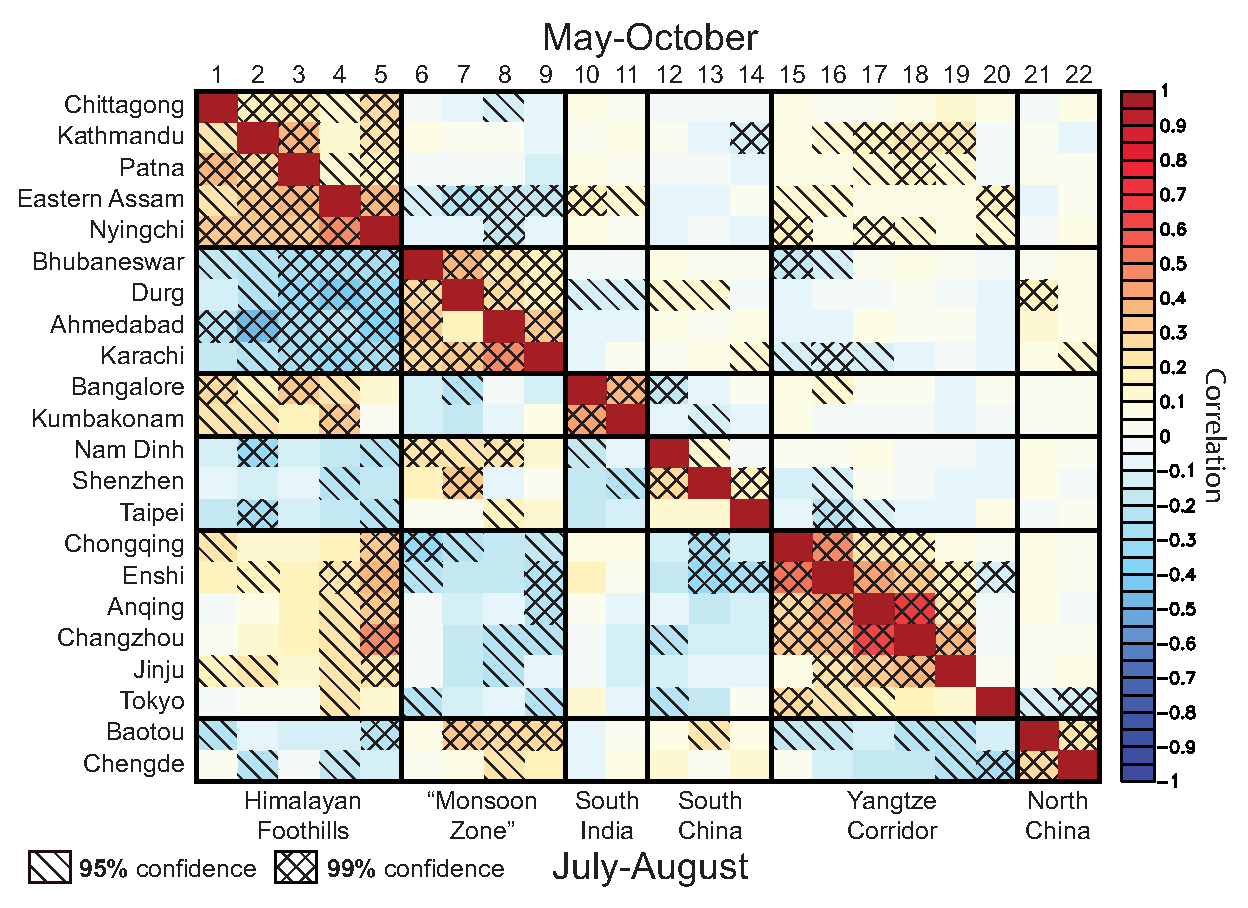
\includegraphics[width=36pc,angle=0]{Figures/ch2/fig3correl}\\
  \caption{Correlation coefficient $r$ of normalized monthly precipitation anomaly time series $P''$ between each of the 22 reference points for the years 1951-2007. Each monthly anomaly is treated as an independent time point. Bottom-left: July-August (JA, 114 time points). Upper-right: May-October (MJJASO, 342 time points). Confidence levels above 95\% and 99\% are indicated by single and double diagonal hatches respectively. Given degrees of freedom $n$, the threshold for significance is listed. July-August ($n=112$) - 95\%/99\%: $\lvert r\rvert >.184/.240$. May-October ($n=340$) - 95\%/99\%: $\lvert r\rvert>.106/.139$. Shared autocorrelation between monthly rainfall anomaly time series is small and does not affect the number of effective degrees of freedom. Region-to-region correlations reproduce point-to-point results closely (not shown).}
\label{fig:f23}
\end{figure}

\begin{figure}[t]
  \noindent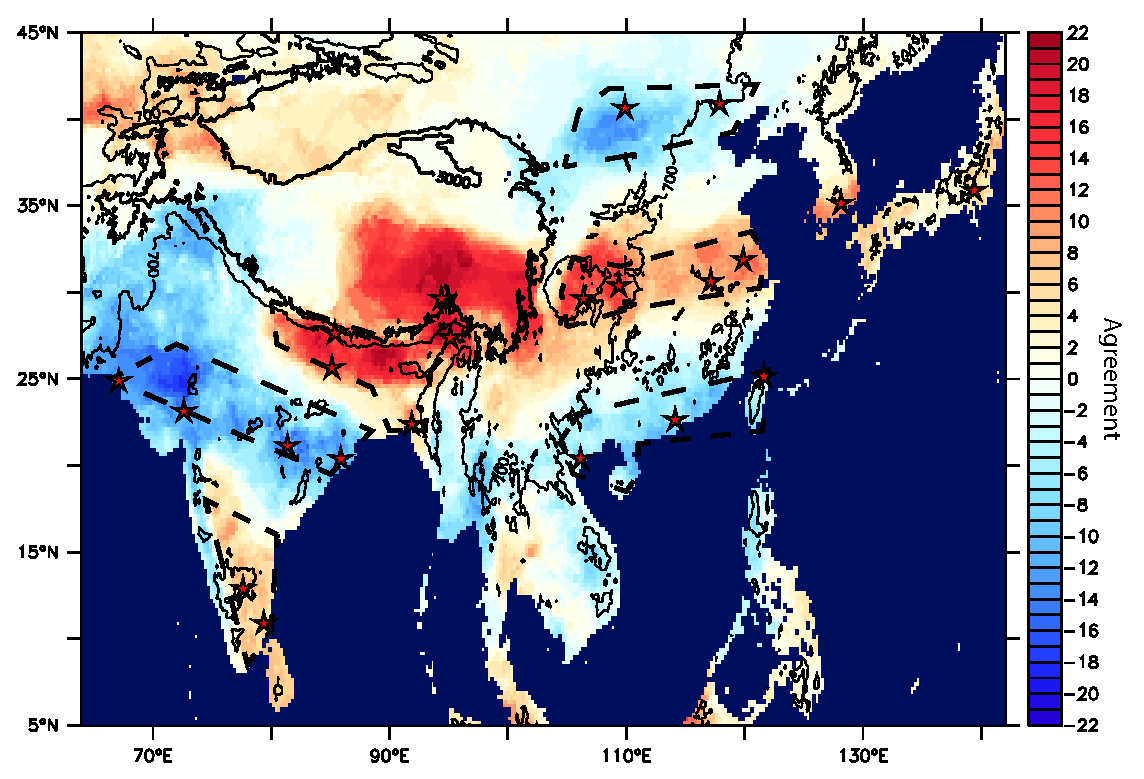
\includegraphics[width=36pc,angle=0]{Figures/ch2/fig4agreement}\\
  \caption{Agreement map $A(x,y)$ of July-August rainfall anomalies predicted by all 22 reference points, calculated using method described in Section 3b, with 3000 meter and 700 meter topography isolines superimposed (thick and thin lines respectively) and reference points marked with red stars.}
  \label{fig:f24}
\end{figure}

\begin{figure}[t]
  \noindent\includegraphics[width=36pc,angle=0]{Figures/ch2/figS1_eof_season}\\
  \caption{EOF 1 of normalized anomaly precipitation for the region 64E-142E and 5N-45N for June through September separately with .5\textdegree\ $\times$ .5\textdegree\ resolution.}
  \label{fig:S21}
\end{figure}

\begin{figure}[t]
  \noindent\includegraphics[width=36pc,angle=0]{Figures/ch2/fig5eof_monthly}\\
  \caption{EOF1 of normalized anomaly precipitation computed separately for June, July, August and September (units of standard deviation) for the All-Asia region (68\textdegree E-140\textdegree E and 5\textdegree -45\textdegree N) with .5\textdegree\ $\times$ .5\textdegree\ resolution for 1951-2007. Percentage of variance explained by each EOF is listed alongside.}
  \label{fig:f25}
\end{figure}

\begin{figure}[t]
  \noindent\includegraphics[width=32pc,angle=0]{Figures/ch2/fig6eof_allasia}\\
  \caption{Leading spatial and temporal EOFs of July-August normalized anomaly precipitation $P''$ for the All-Asia region (64\textdegree E-142\textdegree E and 5\textdegree N-45\textdegree N) with .5\textdegree\ $\times$ .5\textdegree\ resolution for 1951-2007 (114 time points). Percentage of variance explained by each EOF is listed alongside. July (white shading) and August (gray shading) value of temporal EOF are shown separately. Time series are normalized to unit variance ($\sigma=1$).}
  \label{fig:f26}
\end{figure}

\begin{figure}[t]
  \noindent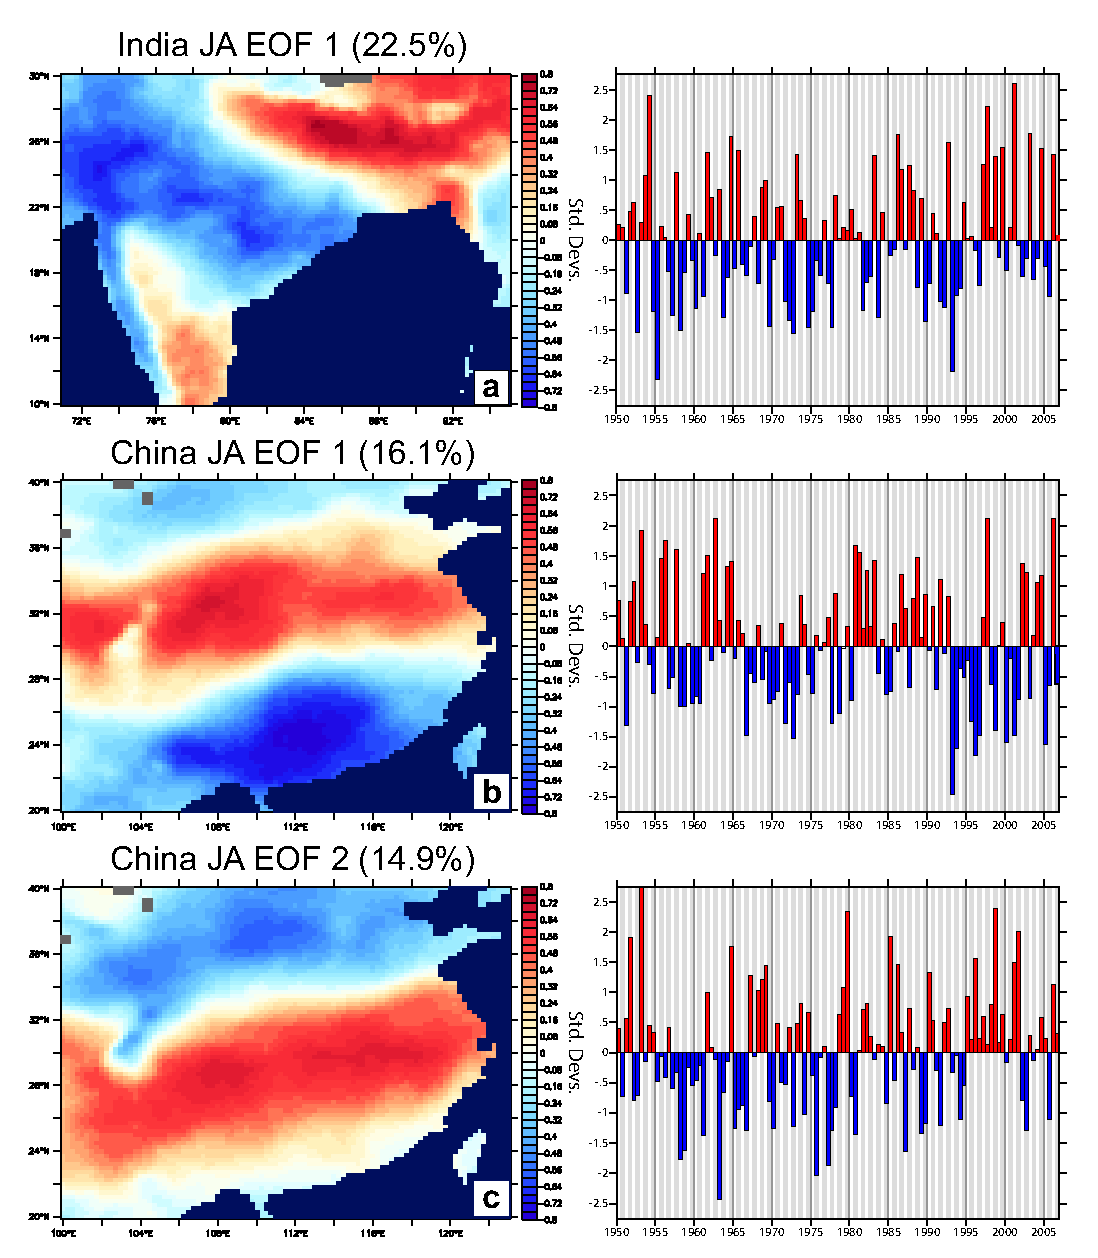
\includegraphics[width=36pc,angle=0]{Figures/ch2/fig7eof_region}\\
  \caption{Leading spatial and temporal EOFs of July-August normalized anomaly precipitation $P''$ for India (71\textdegree E-95\textdegree E and 10\textdegree N-30\textdegree N) and China (100\textdegree E-123\textdegree E and 20\textdegree N-40\textdegree N) with .25\textdegree\ $\times$ .25
  textdegree\ resolution for 1951-2007 (114 time points). Percentage of variance explained by each EOF is listed alongside. July (white shading) and August (gray shading) are both shown. Time series are normalized to unit variance ($\sigma=1$).}\label{fig:f27}
\end{figure}

\begin{figure}[t]
  \noindent\includegraphics[width=42pc,angle=0]{Figures/ch2/fig8laglead}\\
  \caption{July-August $K_i^\lambda$ for reference point $(x_i,y_i)$ (red star) and $\lambda= -5\ \mathrm{ to }\ 5$, where $K_i^\lambda$ is the 57-year mean of anomalous correlation $C_i^\lambda$ of local rainfall $P''(x_i,y_i)$ with normalized anomaly rainfall $P''$ at all other points, with an imposed lag or lead of $\lambda$ days (see main text for formula). Variance circles for a given $\lambda$ are drawn to include at least 50\% of yearly maxima of anomalous correlation $C_i^\lambda$ from all 57 years, with X marking their center.}
  \label{fig:f28}
\end{figure}

\begin{figure}[t]
  \noindent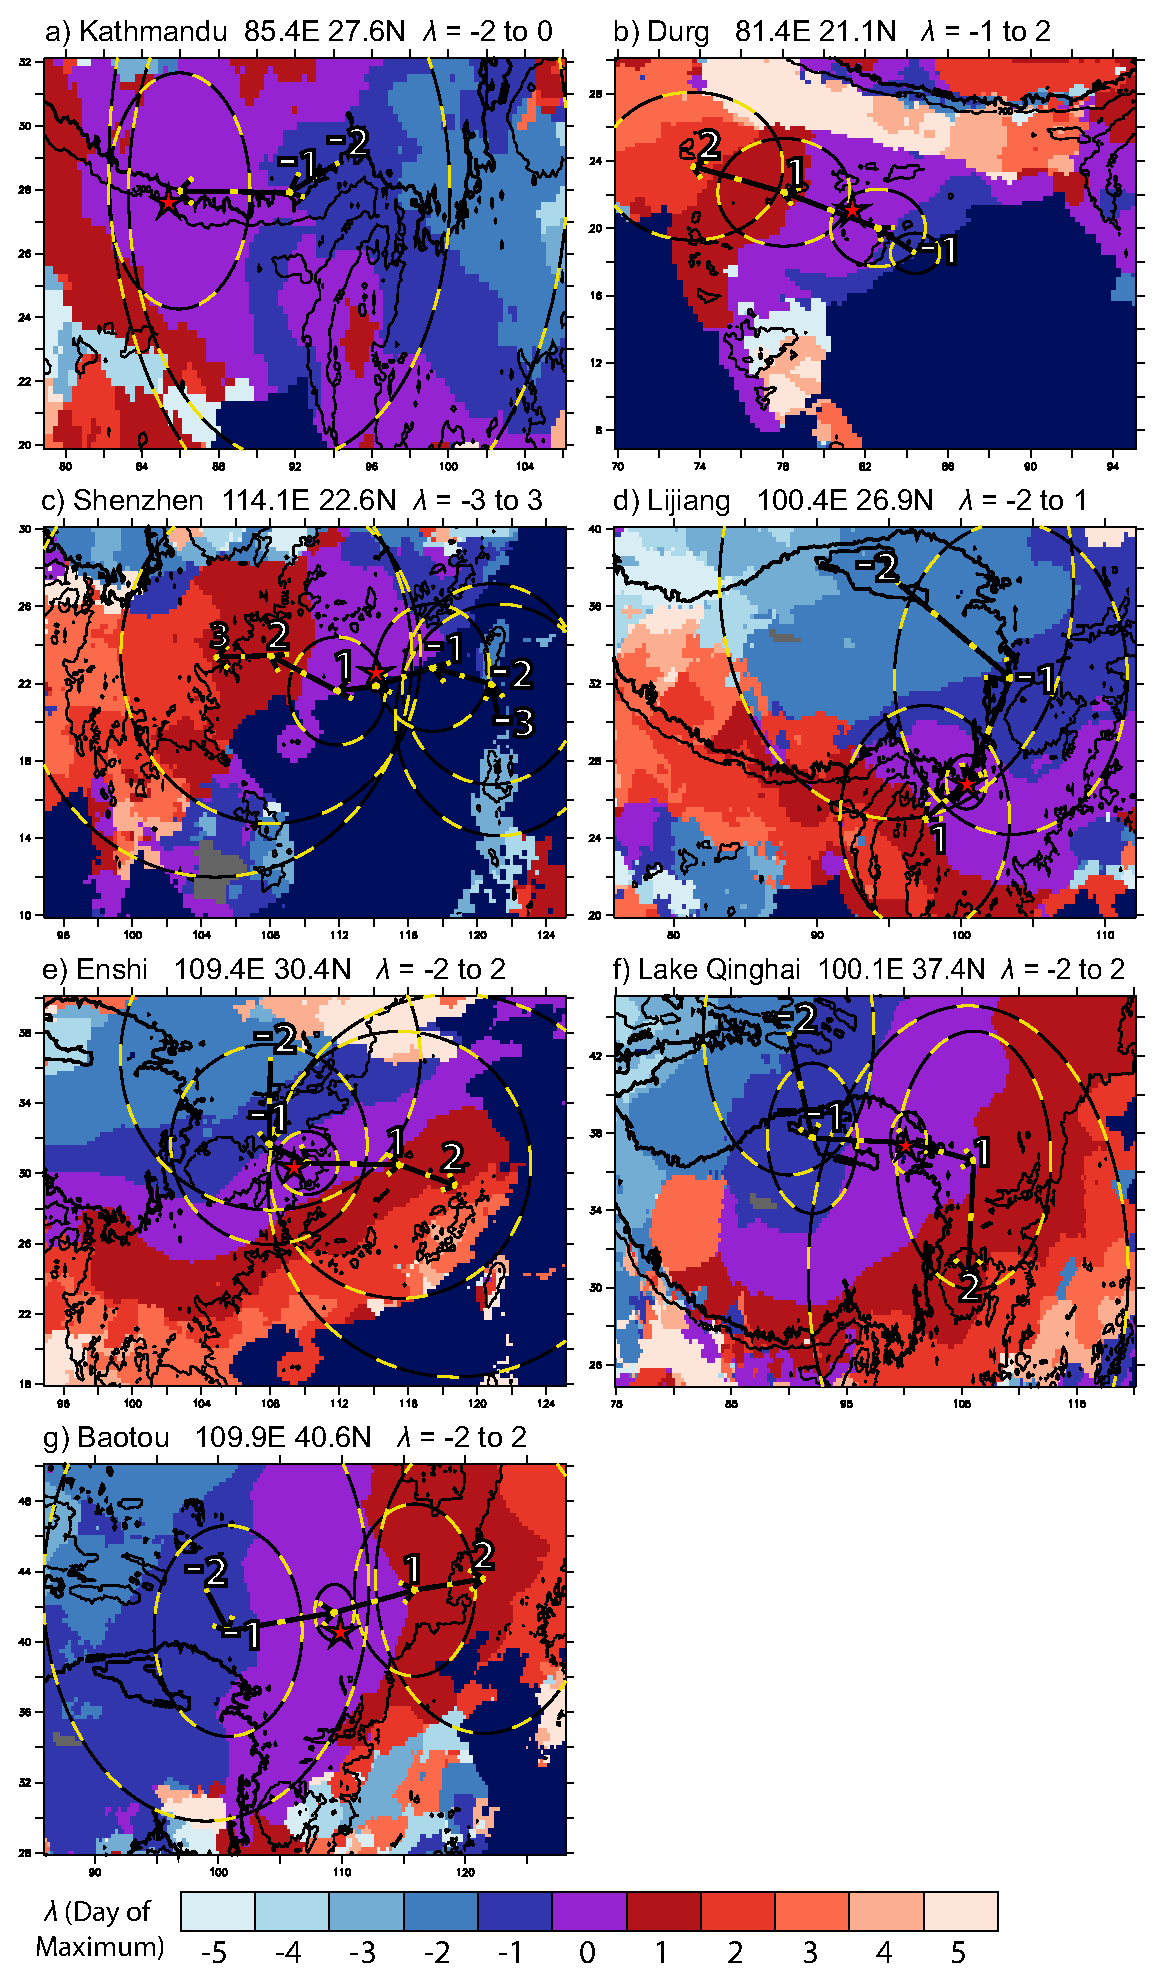
\includegraphics[width=31pc,angle=0]{Figures/ch2/fig9kmax}\\
  \caption{July-August plot of the lag $\lambda$ for which, given listed reference point $(x_i,y_i)$ (red star), the 57-year mean anomalous correlation of rainfall $K_i^\lambda(x,y)$ is maximized. Variance circles from Figure 9 (black with yellow highlights) are superimposed for range of $\lambda$ listed above each figure, with connecting arrows showing propagation (also black with yellow highlights).}
  \label{fig:f29}
\end{figure}

\begin{figure}[t]
  \noindent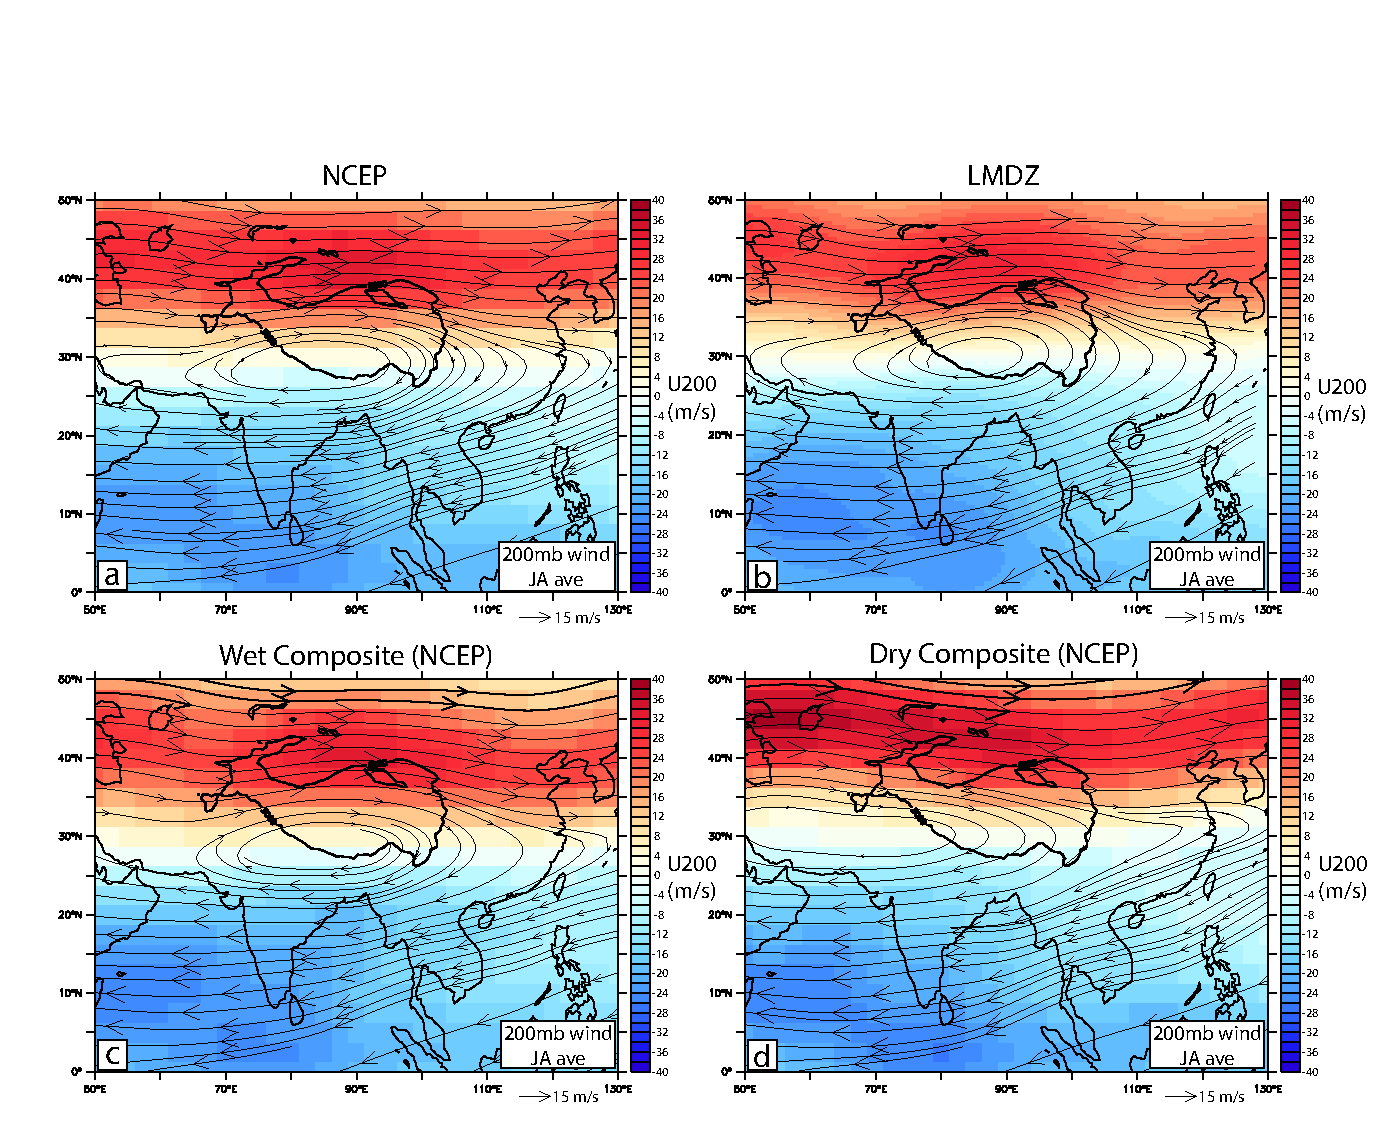
\includegraphics[width=36pc,angle=0]{Figures/ch2/fig10u200}\\
  \caption{July-August streamlines of mean 200 mb level winds from NCEP reanalysis (1948-2014) (a) and LMDZ 200 mb winds for the year 2006 (b). Figures c and d are NCEP reanalysis 200 mb-level wind for composites of ``wet'' years (c) and ``dry'' years (d). The ``wet'' composite includes the five years with the most positive value of All-Asia JA EOF1, while the ``dry'' composite is the equivalent with the five most negative years.}
  \label{fig:f210}
\end{figure}

\begin{figure}[t]
  \noindent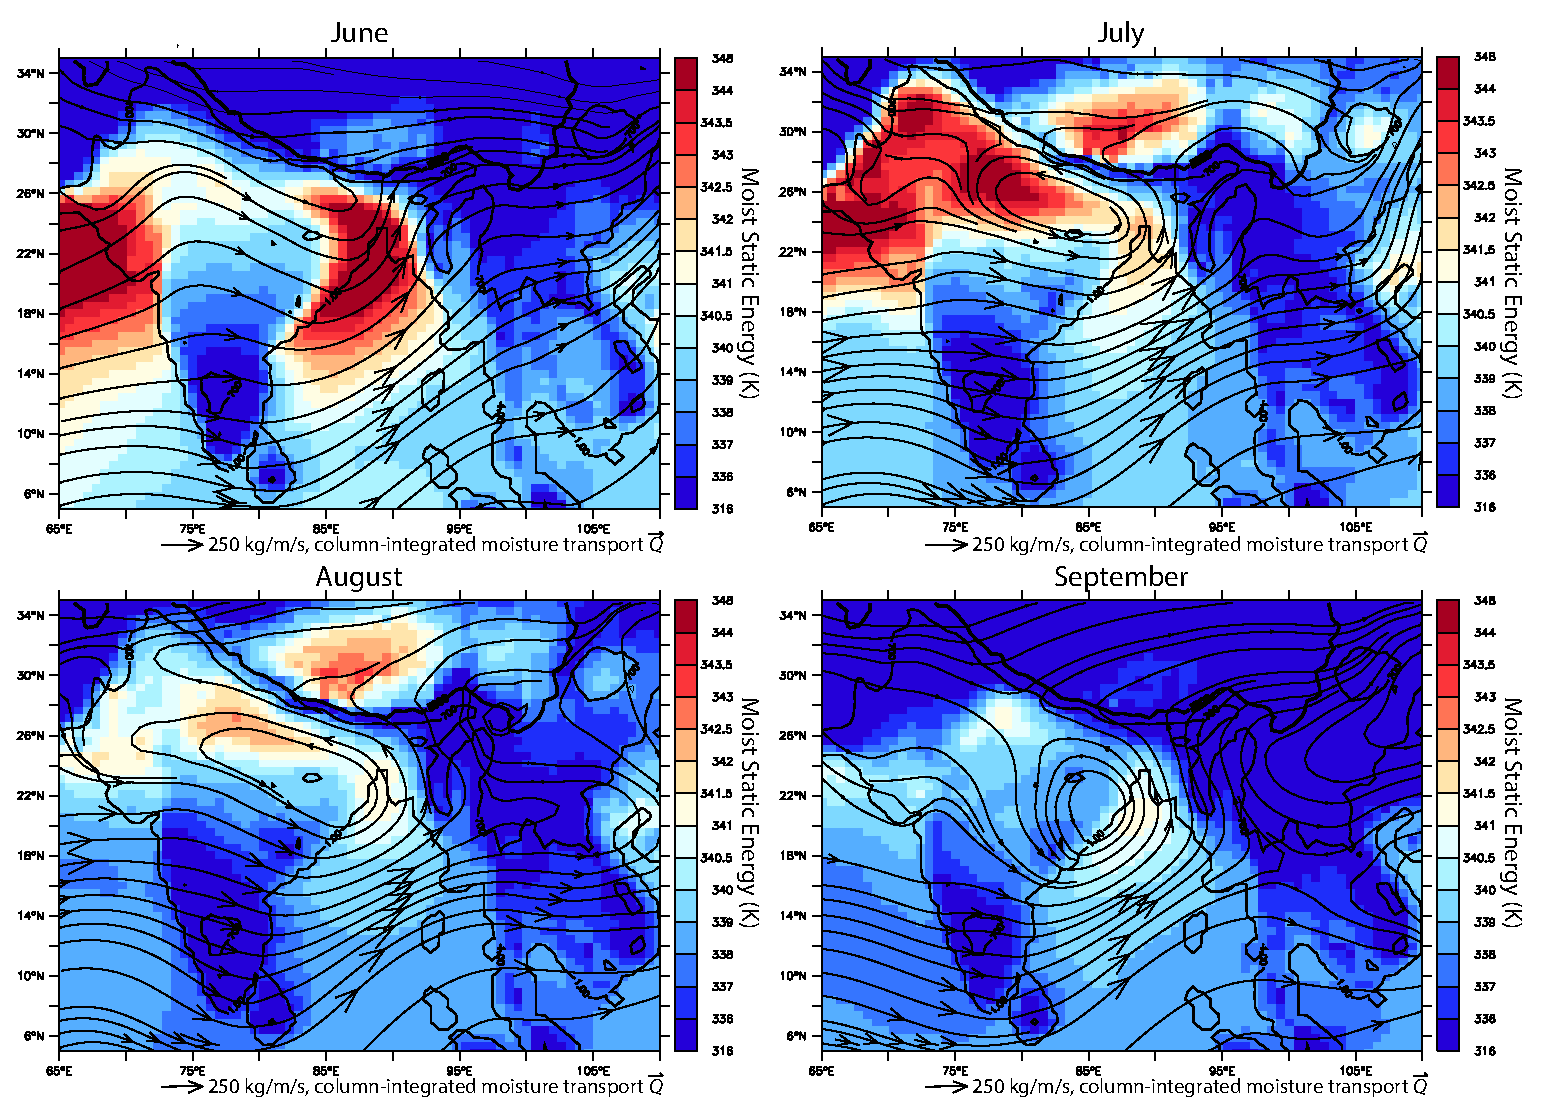
\includegraphics[width=36pc,angle=0]{Figures/ch2/fig11lmdz}\\
  \caption{LMDZ values of near-surface moist static energy $h_b$ (shading) and column-integrated moisture transport $\vec{Q}$ (streamlines, magnitude shown by size of arrowheads) for each month from June to September 2006 over the region 65\textdegree E-110\textdegree E and 5\textdegree N-35\textdegree N. Moist static energy is given by the formula $h_b=c_pT+L_vq+gz$, with specific heat of dry air $c_p$ and latent heat of condensation of water $L_v$, as described in main text. Units of moist static energy are Kelvin, obtained by dividing $h_b$ by $c_p$ as practiced in \cite{Boos2013a}. Column-integrated moisture transport is given by $\vec{Q}=\frac{1}{g}\int q\vec{u}\ \mathrm{d}p $. Note unusual color scale of moist static energy used to emphasize changes over continental India.}
  \label{fig:f211}
\end{figure}
